\chapter{Corrections and Systematic Uncertainties} \label{ch:error}

This large amount of data offers a unique chance to explore jet cross-sections using high statistics.   In order to measure the jet double differential cross-section, the following formula is used,

\begin{equation}
	\frac{d^{2} \sigma^{jet}}{d\eta \, dp_{T}} = \frac{1}{\epsilon_{reco}} \frac{A_{trigger}}{\epsilon_{trigger}(p_{T})} \times C_{MC} \times \frac{1}{A} \times \frac{1}{\mathscr{L}_{int}} \times \frac{dN^{2}_{jet}}{dp_{T} \, d\eta}
\label{eq:xsecdef}
\end{equation}

\noindent
where,

\begin{itemize}
  \item $\epsilon_{reco}$ is the efficency for reconstructing the jet in the ALICE detector.
  \item $A_{trigger}$ is the acceptance for EMCal triggered events and $\epsilon_{trigger}(p_{T})$ is the EMCal trigger efficiency.  These factors correct for imperfections in the electronics of the EMCal and the overall factors are equal to one in Min Bias events.
  \item $C_{MC}$ is a correction factor due to detector effects and it allows for comparisons between the ALICE experiment and other experiments or theoretical calculations.  Unfolding is used to determine this factor.
  \item $\mathscr{L}_{int}$ is the integrated luminosity during the period when the data was recorded.
  \item $A$ is the geometrical detector acceptance.
  \item $\frac{dN^{2}_{jet}}{dp_{T} \, d\eta}$ is the inclusive jet momentum spectra.
  
\end{itemize}

Up to this point I have given an overview of the physics background for jets created in high energy particle collisions, a description of the ALICE detector, and the steps needed to prepare the data for an analysis.  This portion of the thesis will combine all of the data QA together to present a raw jet spectra.  Further cuts for the geometric acceptance, corrections for detector effects, and efficiency calculations need to be accounted for to create a fully corrected jet result.  This chapter will conclude with a presentation of the systematic errors that are reported with the final jet cross-sections

\section{Raw Jet Spectra}

This analysis measured inclusive jet results for radii between 0.1 and 0.5.  However, jet results for radii R = 0.2 to R = 0.4 will be presented in the body of this chapter.  Figures \ref{fig:rawjetR02}, \ref{fig:rawjetR03}, and \ref{fig:rawjetR04} show the raw (uncorrected) $p_{T}$ spectra for inclusive jets from both Min Bias and EMCal triggered data.  It is also evident from these figures that the EMCal triggered data greatly extends the kinematic reach of the measured jet spectra, to about 200 GeV/c.  The EMCal data introduces a bias at low-$p_{T}$ as seen in the different distribution shapes.  The next sections of this chapter will discuss the QA implemented to the data, trigger scaling, unfolding, and other corrections used in this thesis. 

\afterpage{%
\begin{figure}
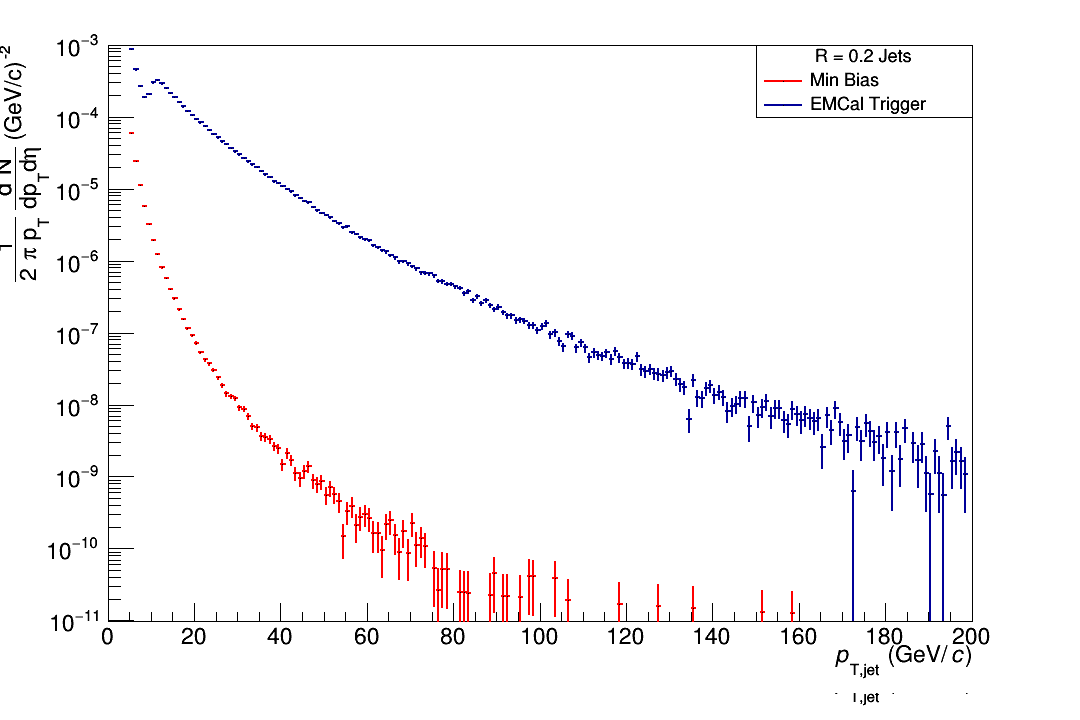
\includegraphics[width=\linewidth]{RawR02JetSpectra}
\centering
\caption{Raw inclusive R = 0.2 jet spectra from the 8 TeV Min Bias and EMCal triggered data}
\label{fig:rawjetR02}
\end{figure}

\begin{figure}
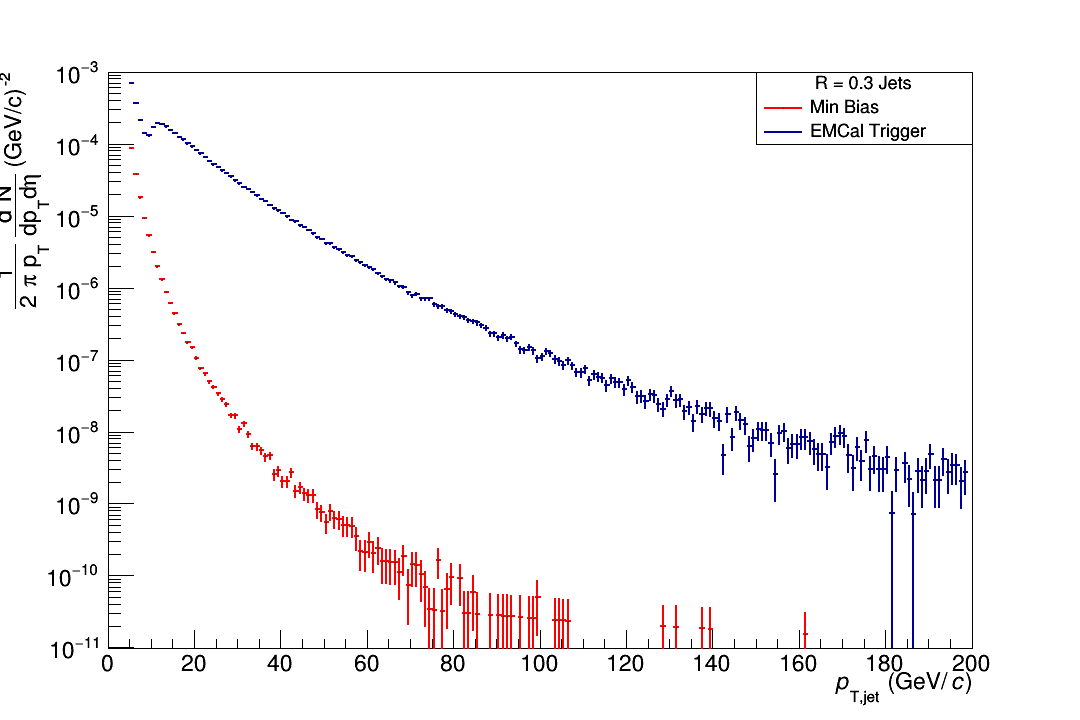
\includegraphics[width=\linewidth]{RawR03JetSpectra}
\centering
\caption{Raw inclusive R = 0.3 jet spectra from the 8 TeV Min Bias and EMCal triggered data}
\label{fig:rawjetR03}
\end{figure}

\begin{figure}
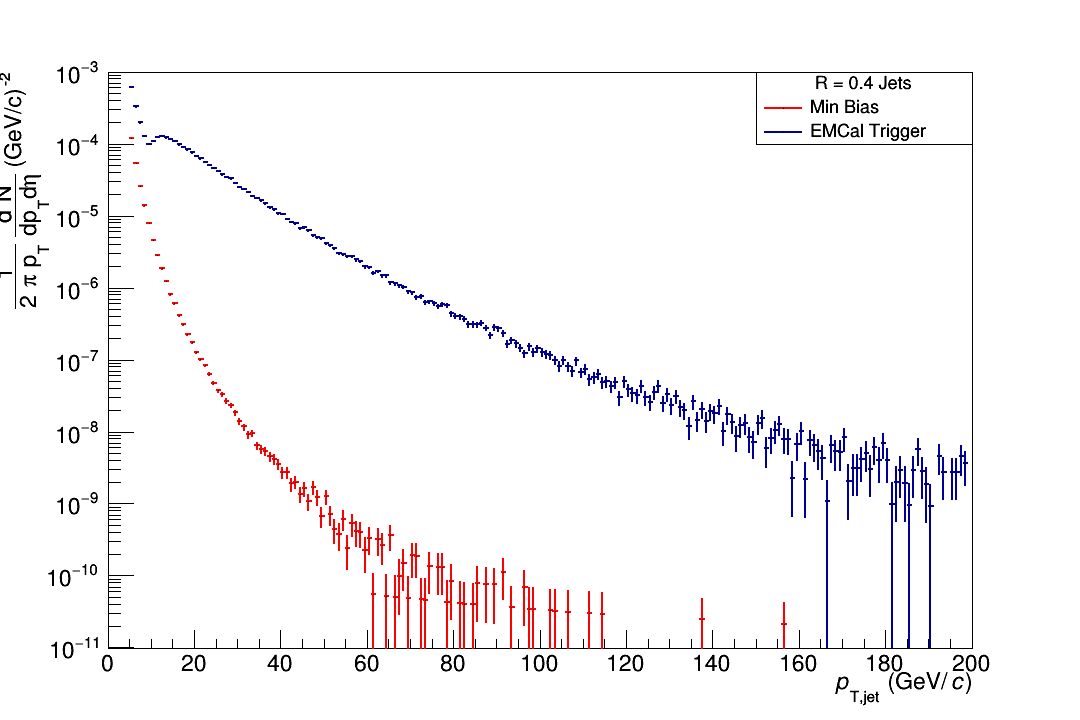
\includegraphics[width=\linewidth]{RawR04JetSpectra}
\centering
\caption{Raw inclusive R = 0.4 jet spectra from the 8 TeV Min Bias and EMCal triggered data}
\label{fig:rawjetR04}
\end{figure}

\clearpage
}


\section{Acceptance Correction}
Jet spectra, cross-sections, and ratios of cross-sections are reported over the full azimuth angle and psuedorapidity acceptance in this thesis.  However, due to jets being constrained to the EMCal, a geometric factor was used to correct for the limited acceptance of the detector.  This thesis explored jet radii between 0.1 and 0.5, in order to study the effects of wide angle radiation on jet fragmentation.  Jet measurements in heavy-ion collisions use radii, typically of 0.2, to help negate the high multiplicity background.  Due to these geometric corrections the centroid of a jet is constrained to,

\begin{equation}
|\eta_{jet}| \leq 0.7 - R, \; 1.4 + R \leq \phi_{jet} \leq 3.14 -R.
\label{eq:jetconstration}
\end{equation}

\begin{equation}
A(p_{T}) = \frac{(1.4 - 2R) \times (1.745 - 2R)}{2 \pi}.
\label{eq:acceptance}
\end{equation}

For jets between R = 0.1 through R = 0.5 the following jet acceptance corrections were used, see Table 5.2.

\begin{table}[hb]
\label{tab:AcceptanceFactor}
\begin{center}
\caption{EMCal jet acceptance for radii 0.1 - 0.5.}
\begin{tabular}[b]{|c|c|c|}
	\hline
	Jet R & $ A $ \\ \hline
	0.1 & 0.296 \\ \hline
	0.2 & 0.214\\ \hline
	0.3 & 0.146\\ \hline
	0.4 & 0.091\\ \hline
	0.5 & 0.048\\ \hline
\end{tabular}
\end{center}

\end{table}

\section{EMCal Triggered Data and Scaling}

The EMCal triggered data for the 8 TeV data greatly extends the kinematic reach for the spectra.  This thesis looked at the two primary Level-1 triggers configured for the EMCal, the jet trigger (EJE) and the gamma (EGA) trigger\cite{Bourrion:2010js}.  Although both of the Level-1 triggers were investigated in this analysis, only the EGA trigger was ultimately corrected  and used for the final jet cross-sections and spectra.  

The EJE trigger utilizes a trigger patch consisting of 32 x 32 EMCal towers sliding by 8 towers until a patch is reconstructed that meets the minimum predefined trigger energy threshold.  Once this threshold is surpassed the event is recorded and tagged as a EJE triggered event.  A similar procedure is followed for the EGA trigger, but with a smaller patch region of 4 x 4 towers with a sliding window of 2 towers and its own predefined trigger threshold.  

The bump at low-$p_{T}$ seen in Figures \ref{fig:rawjetR02} - \ref{fig:rawjetR04} is the trigger turn on curve and the peak corresponds to the trigger threshold for the EGA trigger.  Ideally, a jet in the EMCal acceptance should fire the EJE trigger and the EGA should fire due to the presence of a photon or electron.  Since the triggers increase the yield of jets measured, the spectra from the triggered data must be corrected and downscaled.  In order to calculate these corrections two pieces of code were developed.  One reconstructs the EMCal and trigger patch geometries and allows a user to set the trigger thresholds for the EJE and EGA triggers to values used during a given LHC data taking period.  The other code attempts to match the reconstructed trigger center to the jet center.  The trigger centroid is obtained using a weighted means method by summing over the number of towers in a patch and dividing this quantity by the energy in each tower.  Both sets of codes are publicly available tp the public and are officially part of ALICE software framework.  For this analysis I used a lose requirement that the EGA or EJE patch center were within the radius of a given jet.  The geometrical matching requirement followed a simple quadratic relationship,,

\begin{equation}
\sqrt{ ( \phi_{jet} - \phi_{EGA, patch} )^{2} + ( \eta_{jet} - \eta_{EGA, patch} )^{2}}  \leq R_{jet} .
\label{eq:triggermatch}
\end{equation}

\begin{figure}[h]
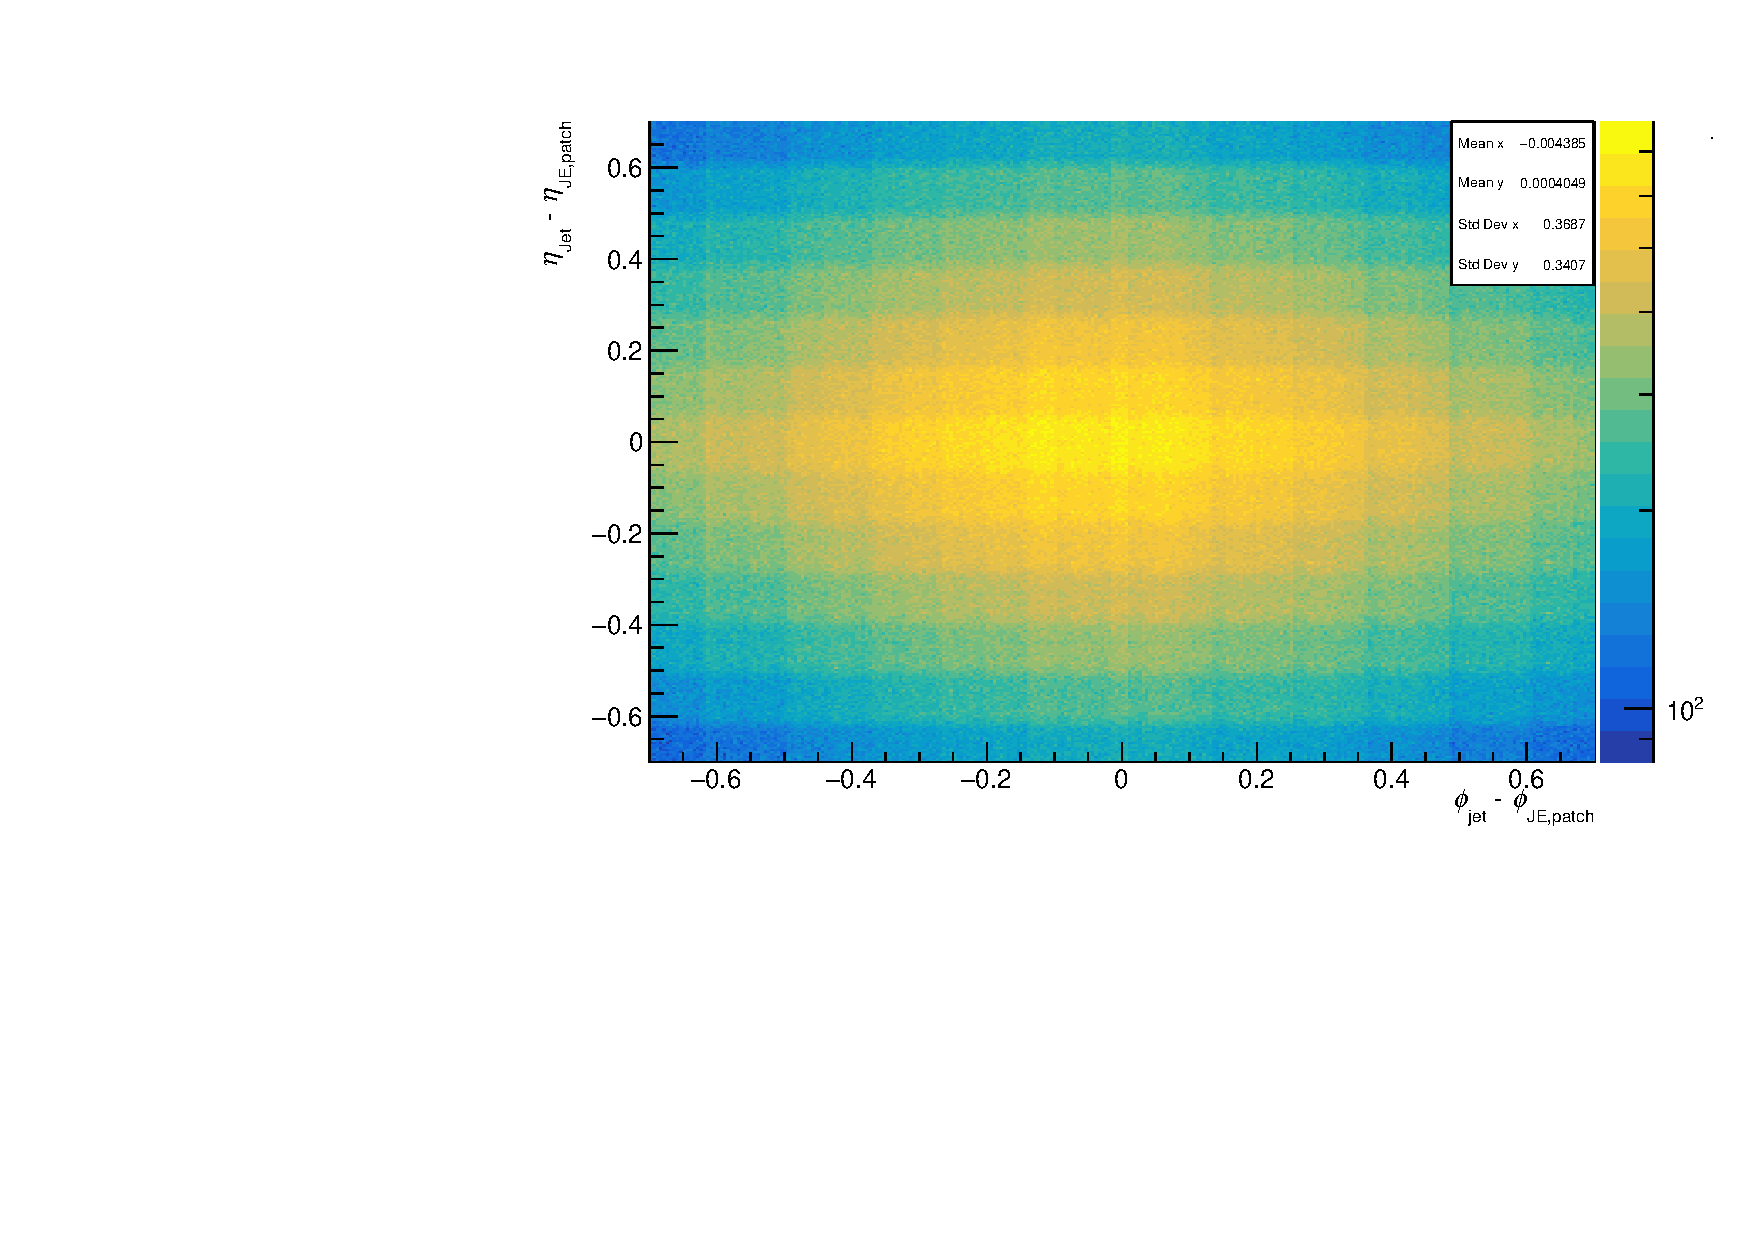
\includegraphics[width=10cm]{DistanceJetEJER02}
\centering
\caption{Distance to closest reconstructed EJE patch to R = 0.2 jet with the Min Bias Pythia Monte Carlo.}
\label{fig:DisJetEJE}
\end{figure}

\begin{figure}[h]
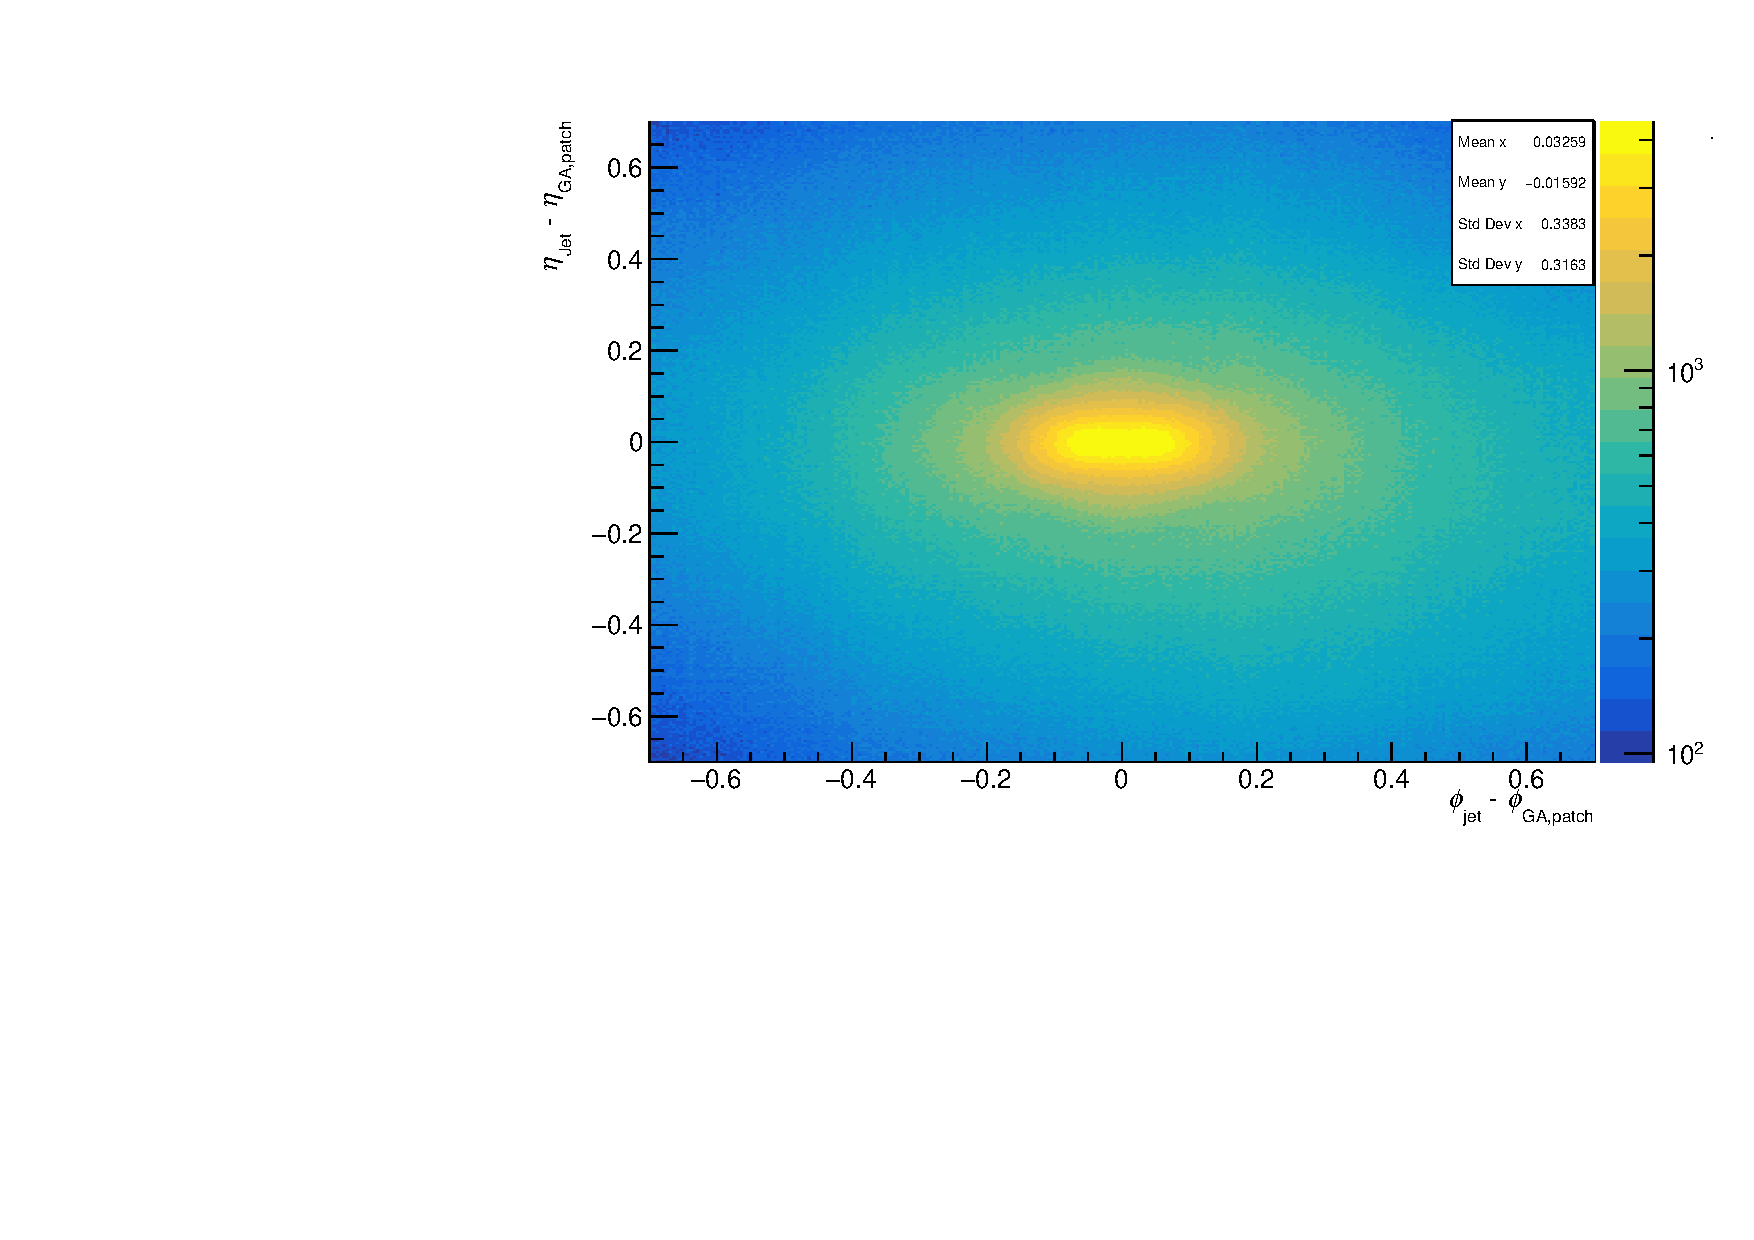
\includegraphics[width=10cm]{DistanceJetEGAR02}
\centering
\caption{Distance to closest reconstructed EGA patch to R = 0.2 jet with the Min Bias Pythia Monte Carlo.}
\label{fig:DisJetEGA}
\end{figure}

\noindent
Figures \ref{fig:DisJetEJE} and \ref{fig:DisJetEGA} show the distance between a reconstructed jet and its closest reconstructed EMCal trigger patch for R = 0.2 jets in the Pythia Monte Carlo.  Since a trigger patch may be fired if two or more jets are within the geometric area of the trigger patch this could lead to double counting.  In order to correct for this, the jet spectra from the triggered data is scaled by the number of triggers, $N_{trig}$, fired that fell within the jet.  We can see that with the EGA trigger that the peak of the distribution is within the jet radius of R = 0.2 while with the EJE trigger the distribution is more uniformly distributed.  The EJE distribution can be accounted for the fact that the EJE trigger is large enough to have multiple jets matched to EJE trigger patch or vice-versa.  The fact that the distribution of seen in Figure \ref{fig:DisJetEJE} spans such a large area means that the jet center was typically not well correlated with the center of the EJE patch and this is the primary reason why the inclusion of the EMCal jet triggered data was abandoned for this thesis.

Once this correction was implemented, the triggered data was then downscaled in order to combine it with the Min Bias data.  The downscale correction factors, shown in Figure \ref{fig:EMCalDownScale}, wee obtained by taking the ratio of the EMCal jet spectra to the Min Bias jet spectra and fitting the plateau region to a line.  At low-$p_{T}$, below $\sim$40 GeV,  the two data sets do not scale linearly and so the EMCal data below 40 GeV was ignored.


\begin{figure*}[t!]
$\begin{array}{rl}
    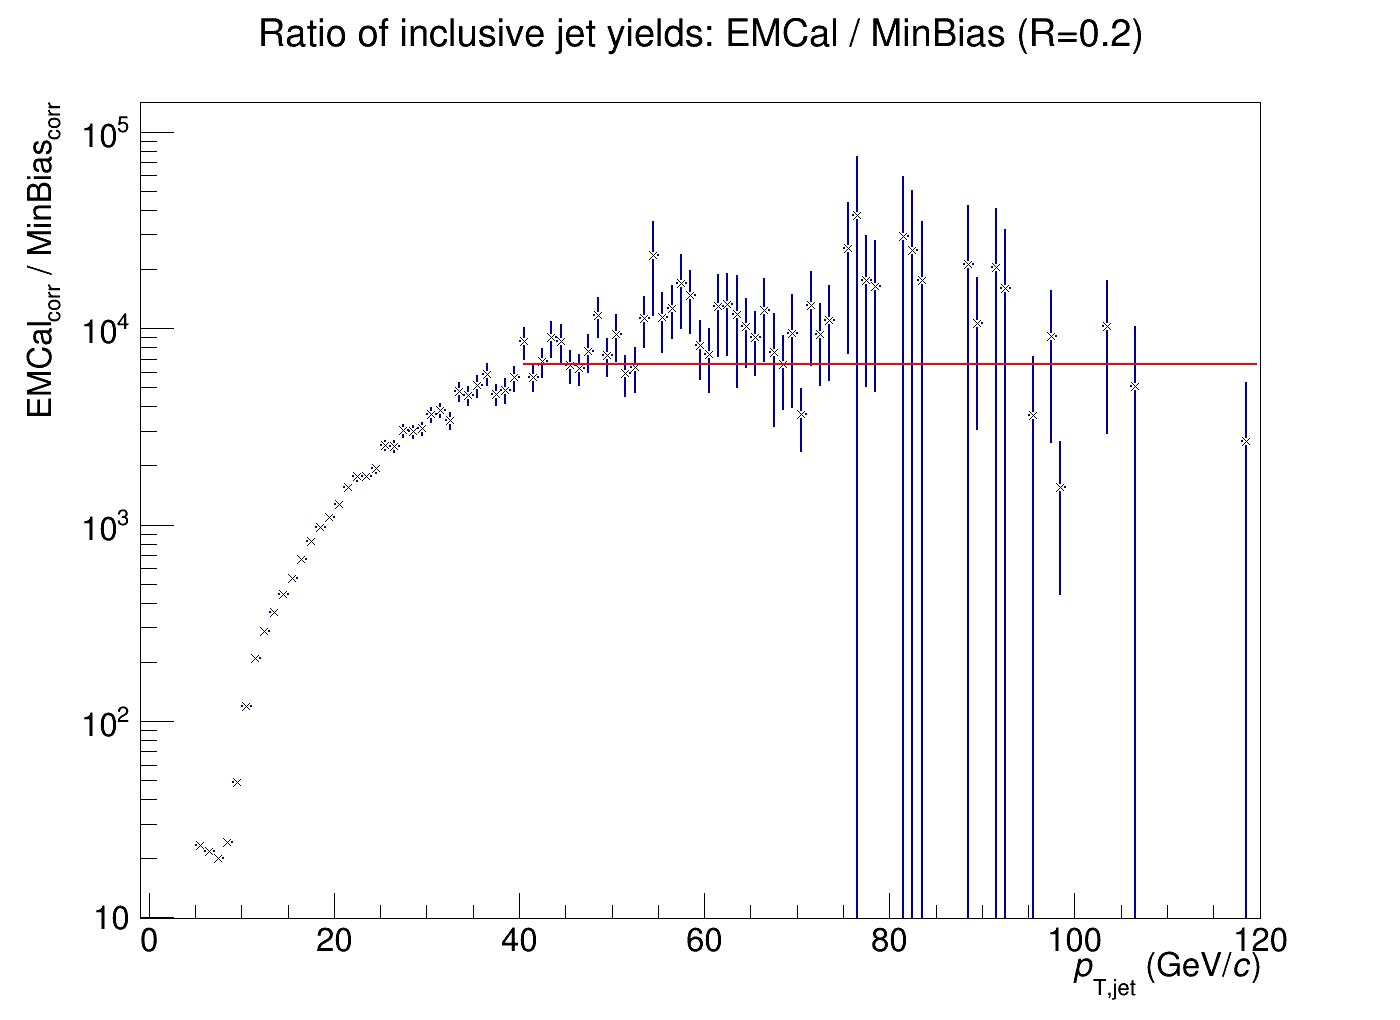
\includegraphics[width=0.5\textwidth]{R02TriggerYields} &
    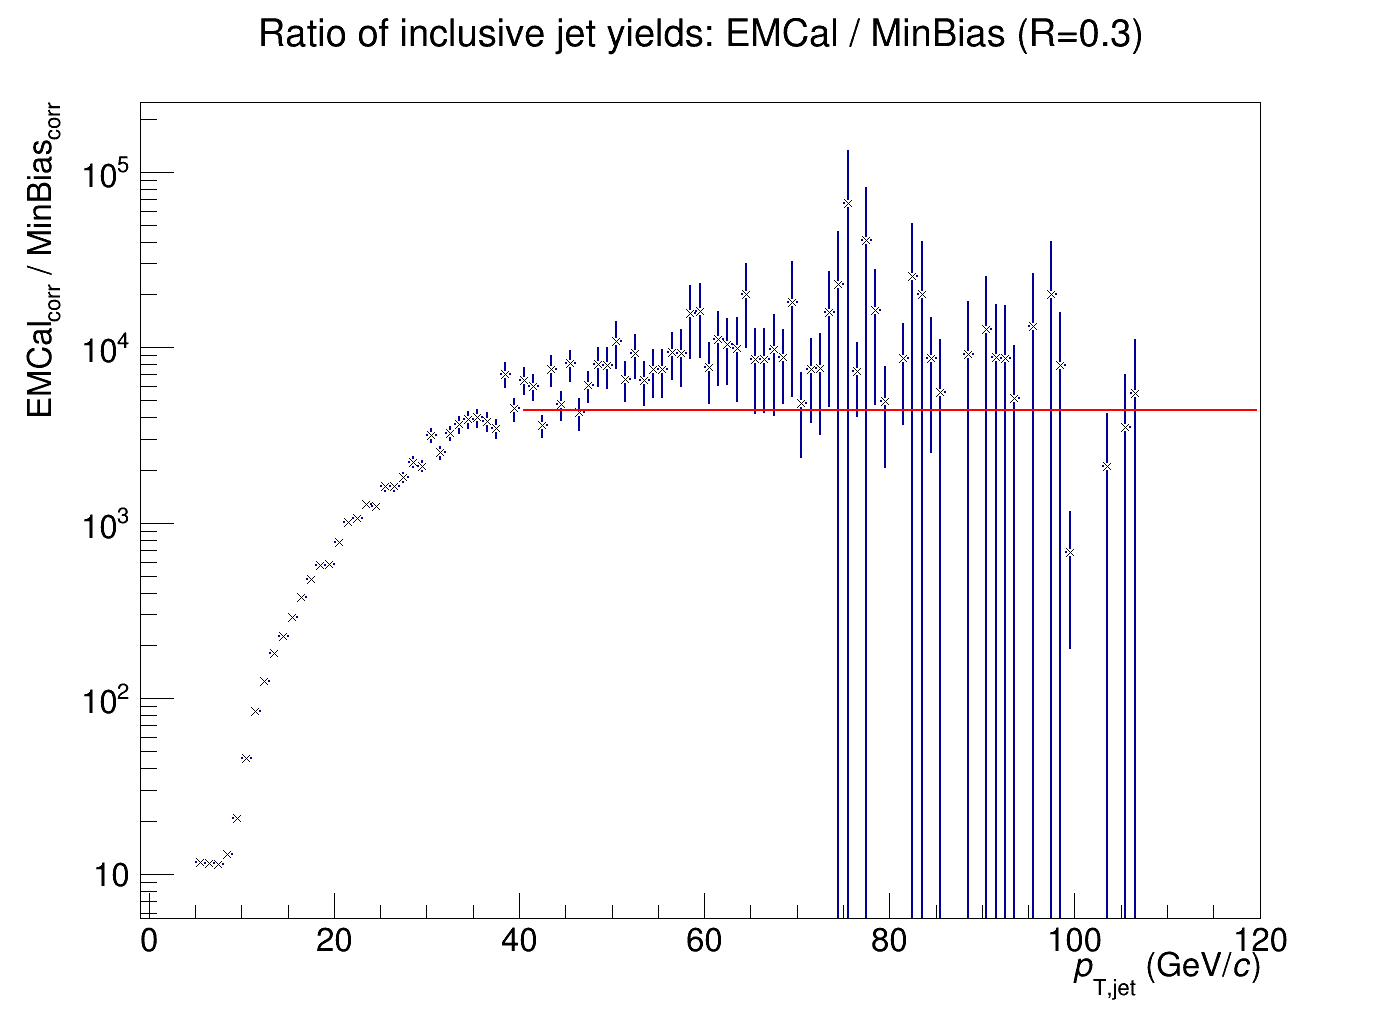
\includegraphics[width=0.5\textwidth]{R03TriggerYields}\\
    \multicolumn{2}{c}{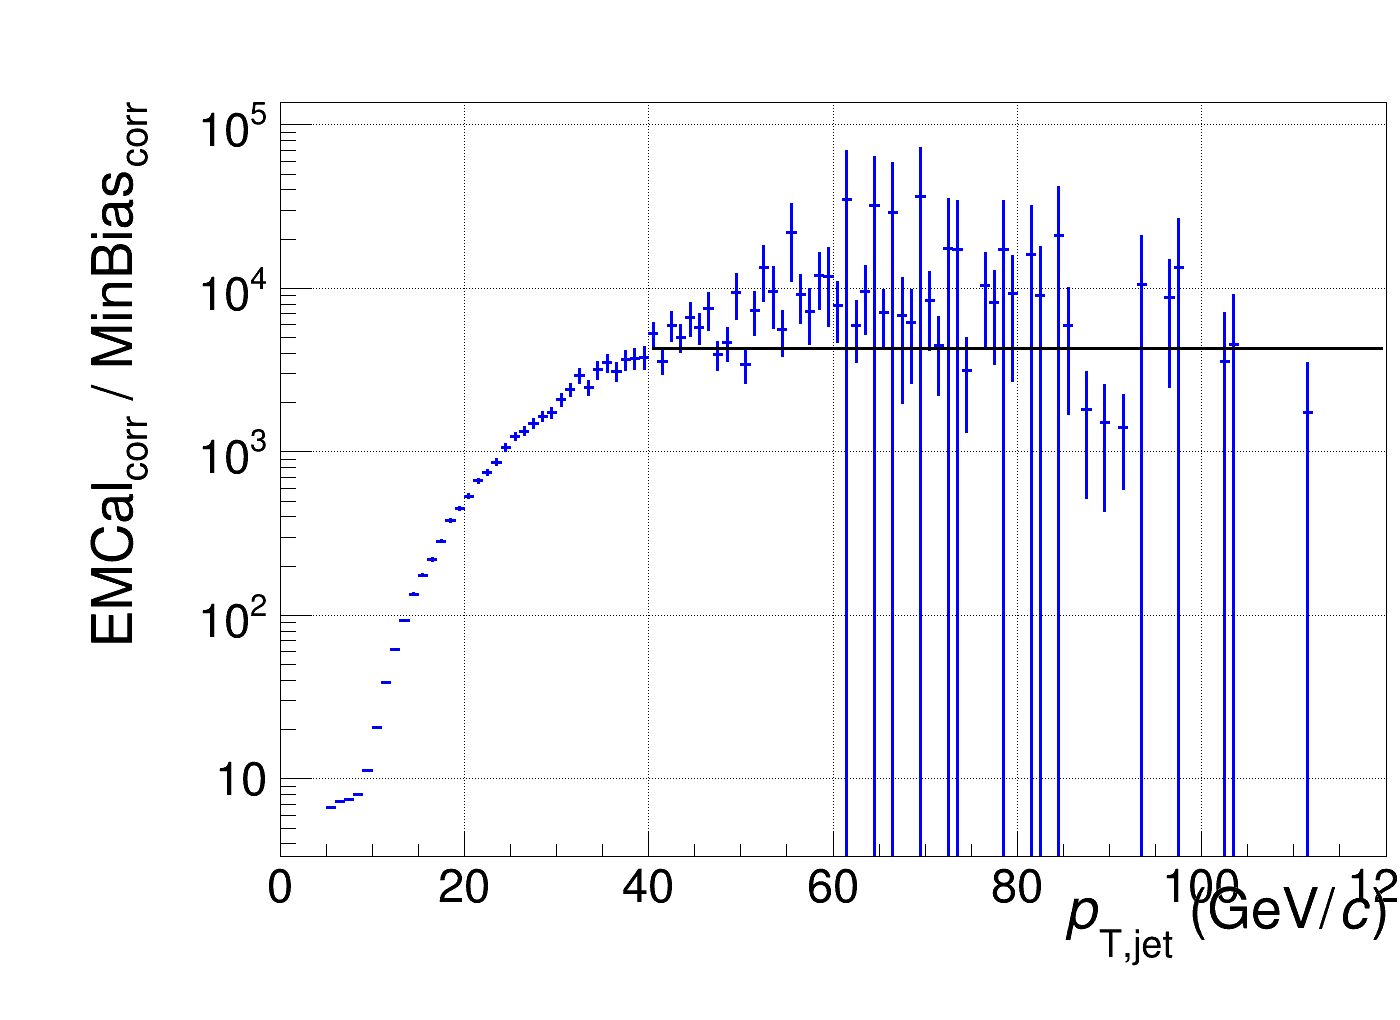
\includegraphics[width=0.5\textwidth]{R04TriggerYields}}
\end{array}$
\caption[EMCal triggered data correction factors for R=0.2, R=0.3, and R=0.4 jets.]{\label{fig:EMCalDownScale}EMCal triggered data correction factors for R=0.2, R=0.3, and R=0.4 jets.}
\end{figure*}

These two corrections allow for the EMCal data to be combined with the Min Bias data.  It should be noted that the scale factors were after the Monte Carlo corrections were implemented which is discussed further on in this chapter.  With the data scaled and combined the next sections will detail more of the QA performed for this analysis.

\section{Corrections to Monte Carlo}

The reconstructed jet $p_{T}$ has a number of detector effects `folded' into the measurement.  These effects included such things as:

\begin{itemize}
\item Tracking inefficiencies from the TPC and ITS.
\item Missing jet energy components from long-lived particles, such as the $K^{0}_{L}$ and neutron, that are cut by the EMCal timing requirement.
\item TPC track $p_{T}$ and EMCal cluster energy resolutions.
\item Hadronic corrections to the EMCal cluster spectrum.
\item Material loss in the detectors.
\end{itemize}

\noindent
Unfolding is a method by which these detector effects are removed from the raw inclusive jet spectra so that a `true' jet spectra may be obtained and compared with theoretical calculations or other experimental results.  

In order to unfold a jet spectra, it is necessary to generate a response matrix that simulates the described effects above.  After the response matrix is generated a number of statistical approaches including, Bayesian, Singular Value Decomposition (SVD), or Bin-by-Bin, may be applied to unfold the raw jet spectra.  In order to generate the response matrix, a Pythia generated event is embedded into a GEANT simulation of the ALICE detector.  Due to the fact that the performance and efficiency of the ALICE detector may change between the data taking periods each simulation is `anchored' to a given LHC.  These anchors contain all the hot and dead sectors for the subdetectors, along with their calibrated performance during that specified data taking.  Two Monte Carlo data sets were produced with the Min Bias trigger simulated for the full 8 TeV run, the first was a Pythia generator using the Monesh-2013 tune and the second was a Min Bias tune of the PHOjet Monte Carlo package.  Both data sets were explored for this thesis and it was decided that the final corrected spectra would be obtained via unfolding with the Pythia Monte Carlo data set.  The magnitude of any one of the effects unfolding is supposed to account for is not expected to be very large, but combined may be significant, thus unfolding is an important step in this analysis.

\subsubsection{Response Matrix}
Given a truth-level, the Monte Carlo event at the particle level, jet $p_{T}$ we wish to reconstruct that jet's $p_{T}$ at the detector-level.  The particle-level Pythia jets are constructed from the primary particles generated via Pythia, while excluding any daughter decay particles in order to avoid double counting.  In addition the tracking efficiency in Pythia is known to deviate from nature.  This is due to Pythia under predicting the production of strange quarks.  
Constructing the response matrix in this case was calculated on a jet-by-jet basis.  The particle-level jet centroid ($\phi_{part}$,$\eta_{part}$)is matched to the detector-level jet via a constrain on the displaced distance between the two jet centroids in ($\phi$,$\eta$).  This distance was constrained to: $\Delta  R = \sqrt{(\phi_{part} - \phi_{det})^{2} + (\eta_{part} - \eta_{det})^{2}} \leq 0.25 \; $.  Once a jet was matched at the detector level to a jet generated from the particle level the response matrix was incremented by jet $p_{T}$ at both the detector and Monte Carlo levels.  The response matrix was generated with a fine binning width of 1 GeV. 

\begin{figure*}[t!]
$\begin{array}{rl}
    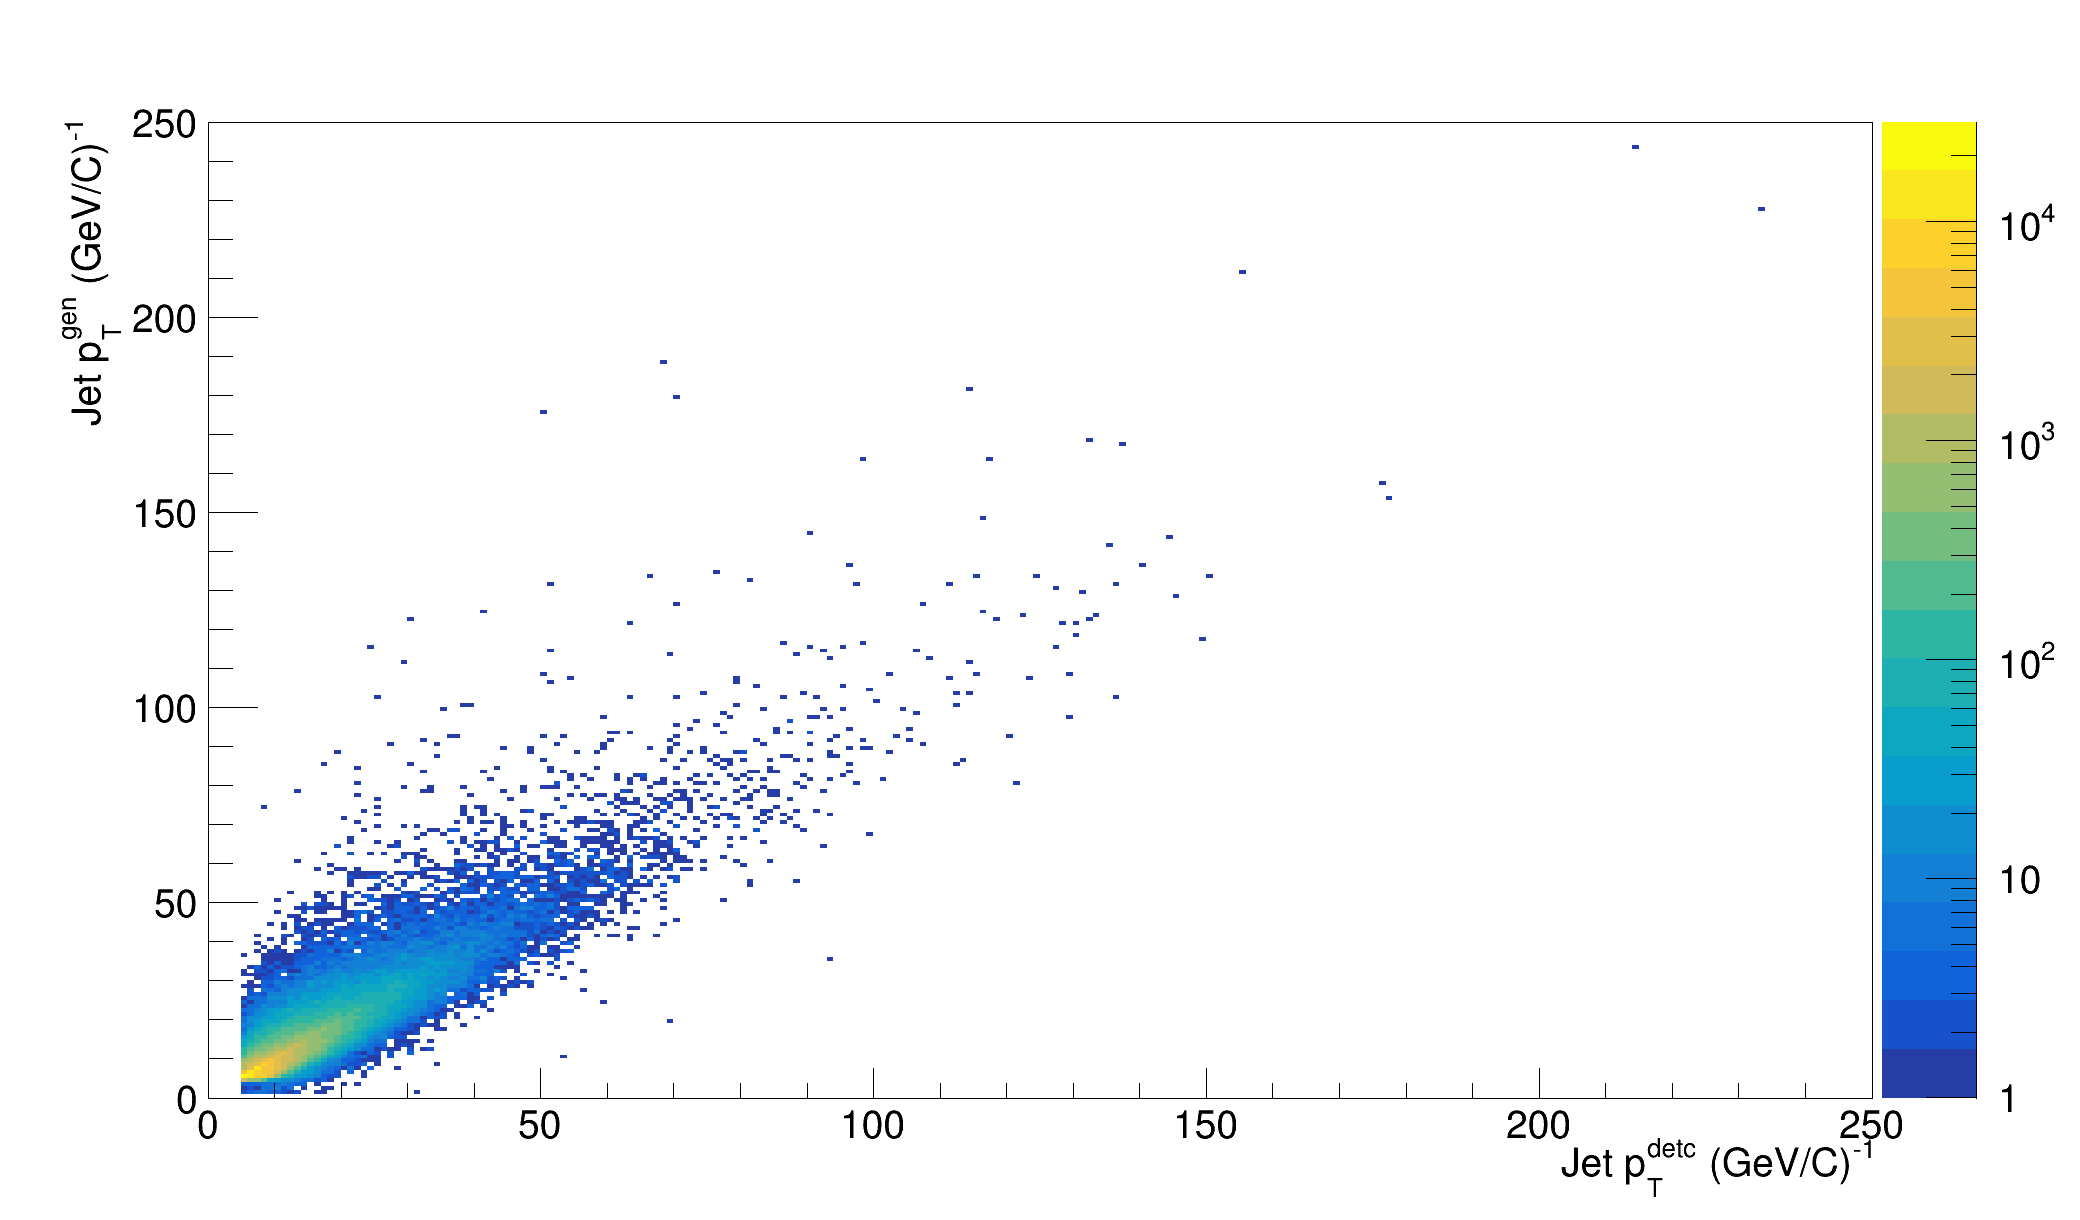
\includegraphics[width=0.5\textwidth]{responseR02} &
    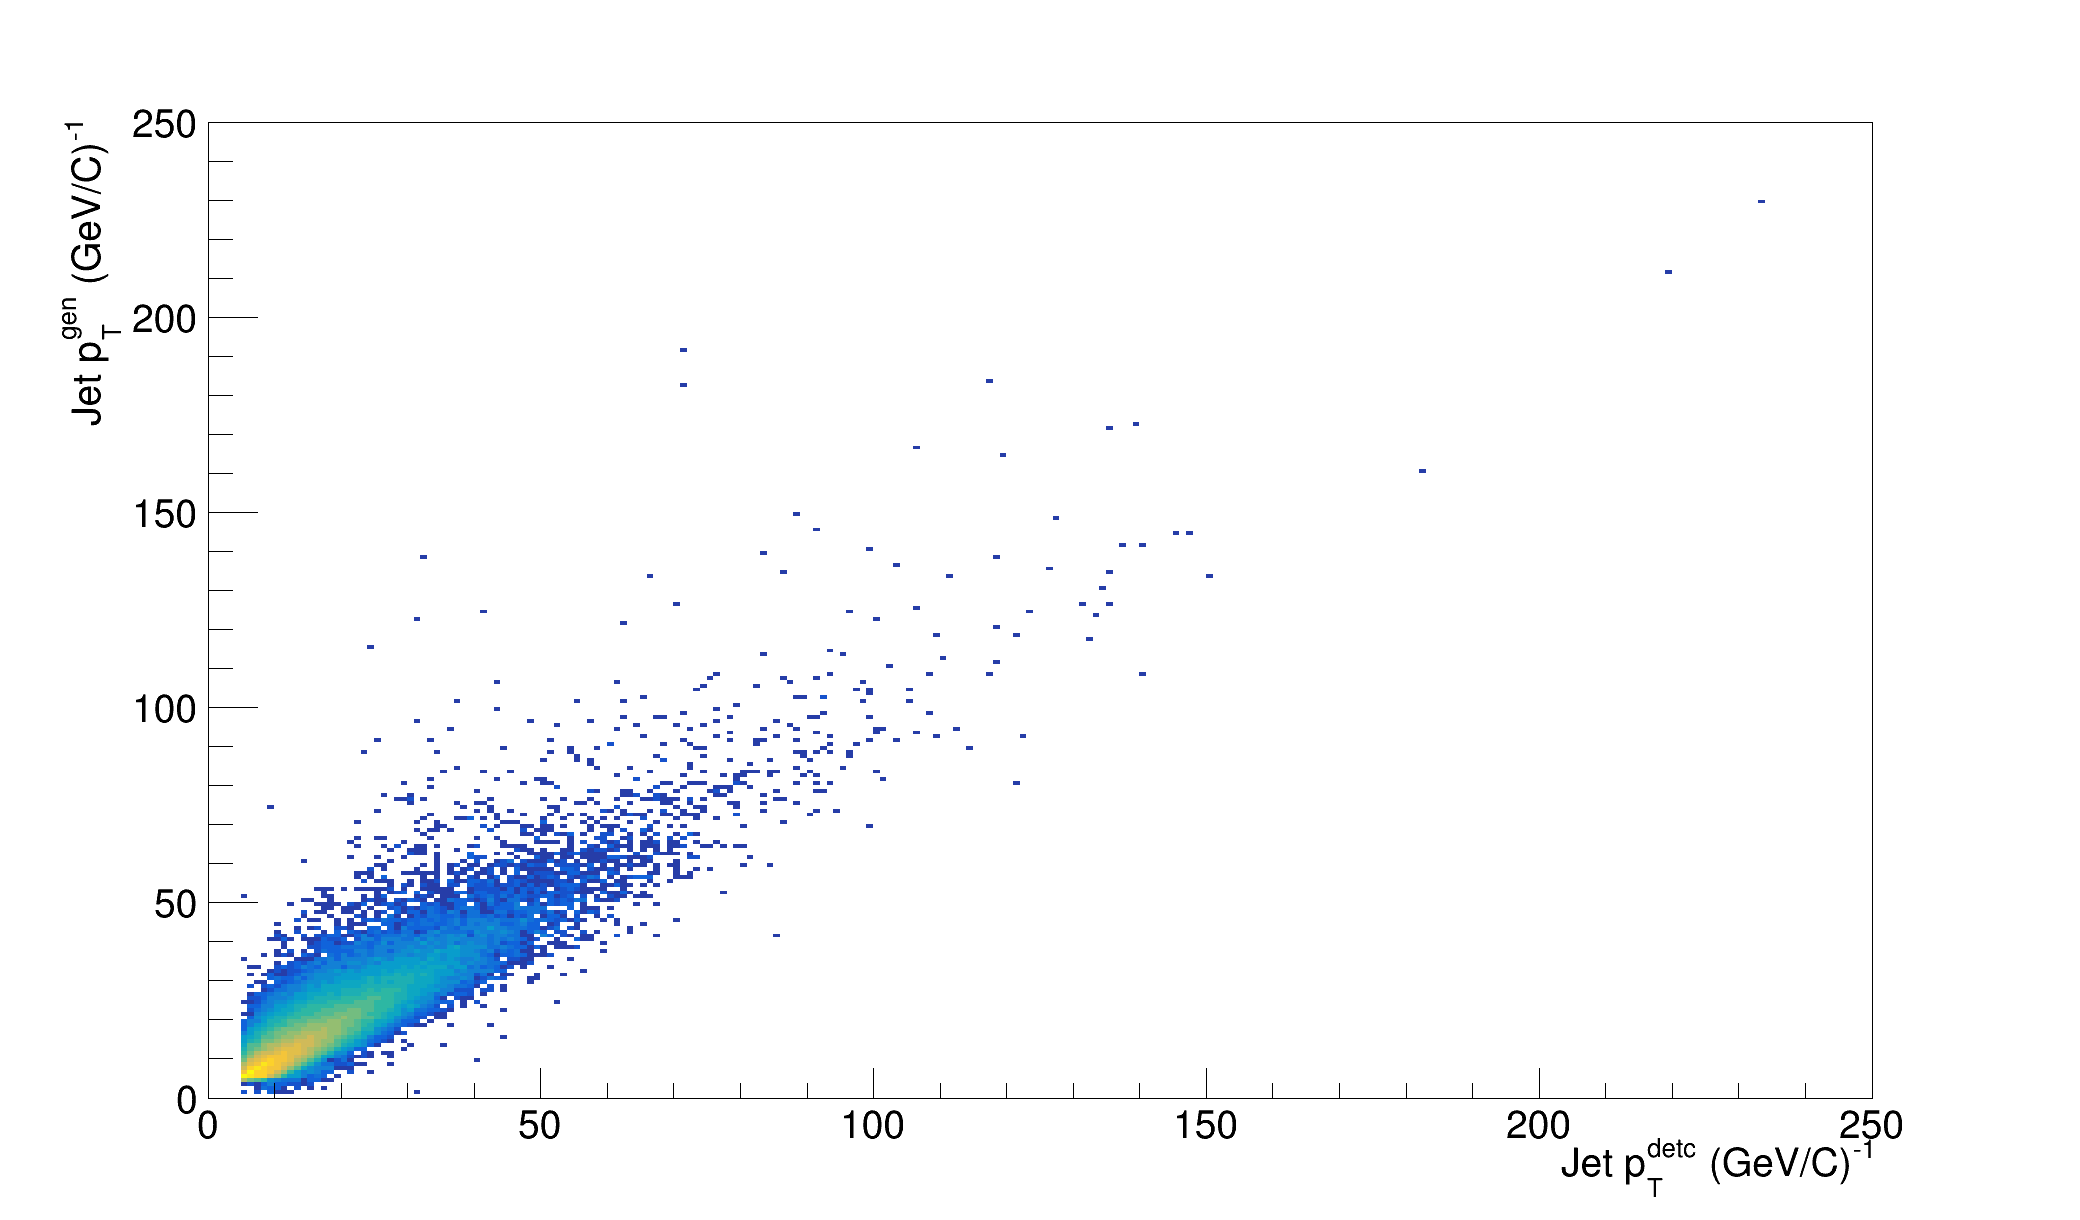
\includegraphics[width=0.5\textwidth]{responseR03}\\
    \multicolumn{2}{c}{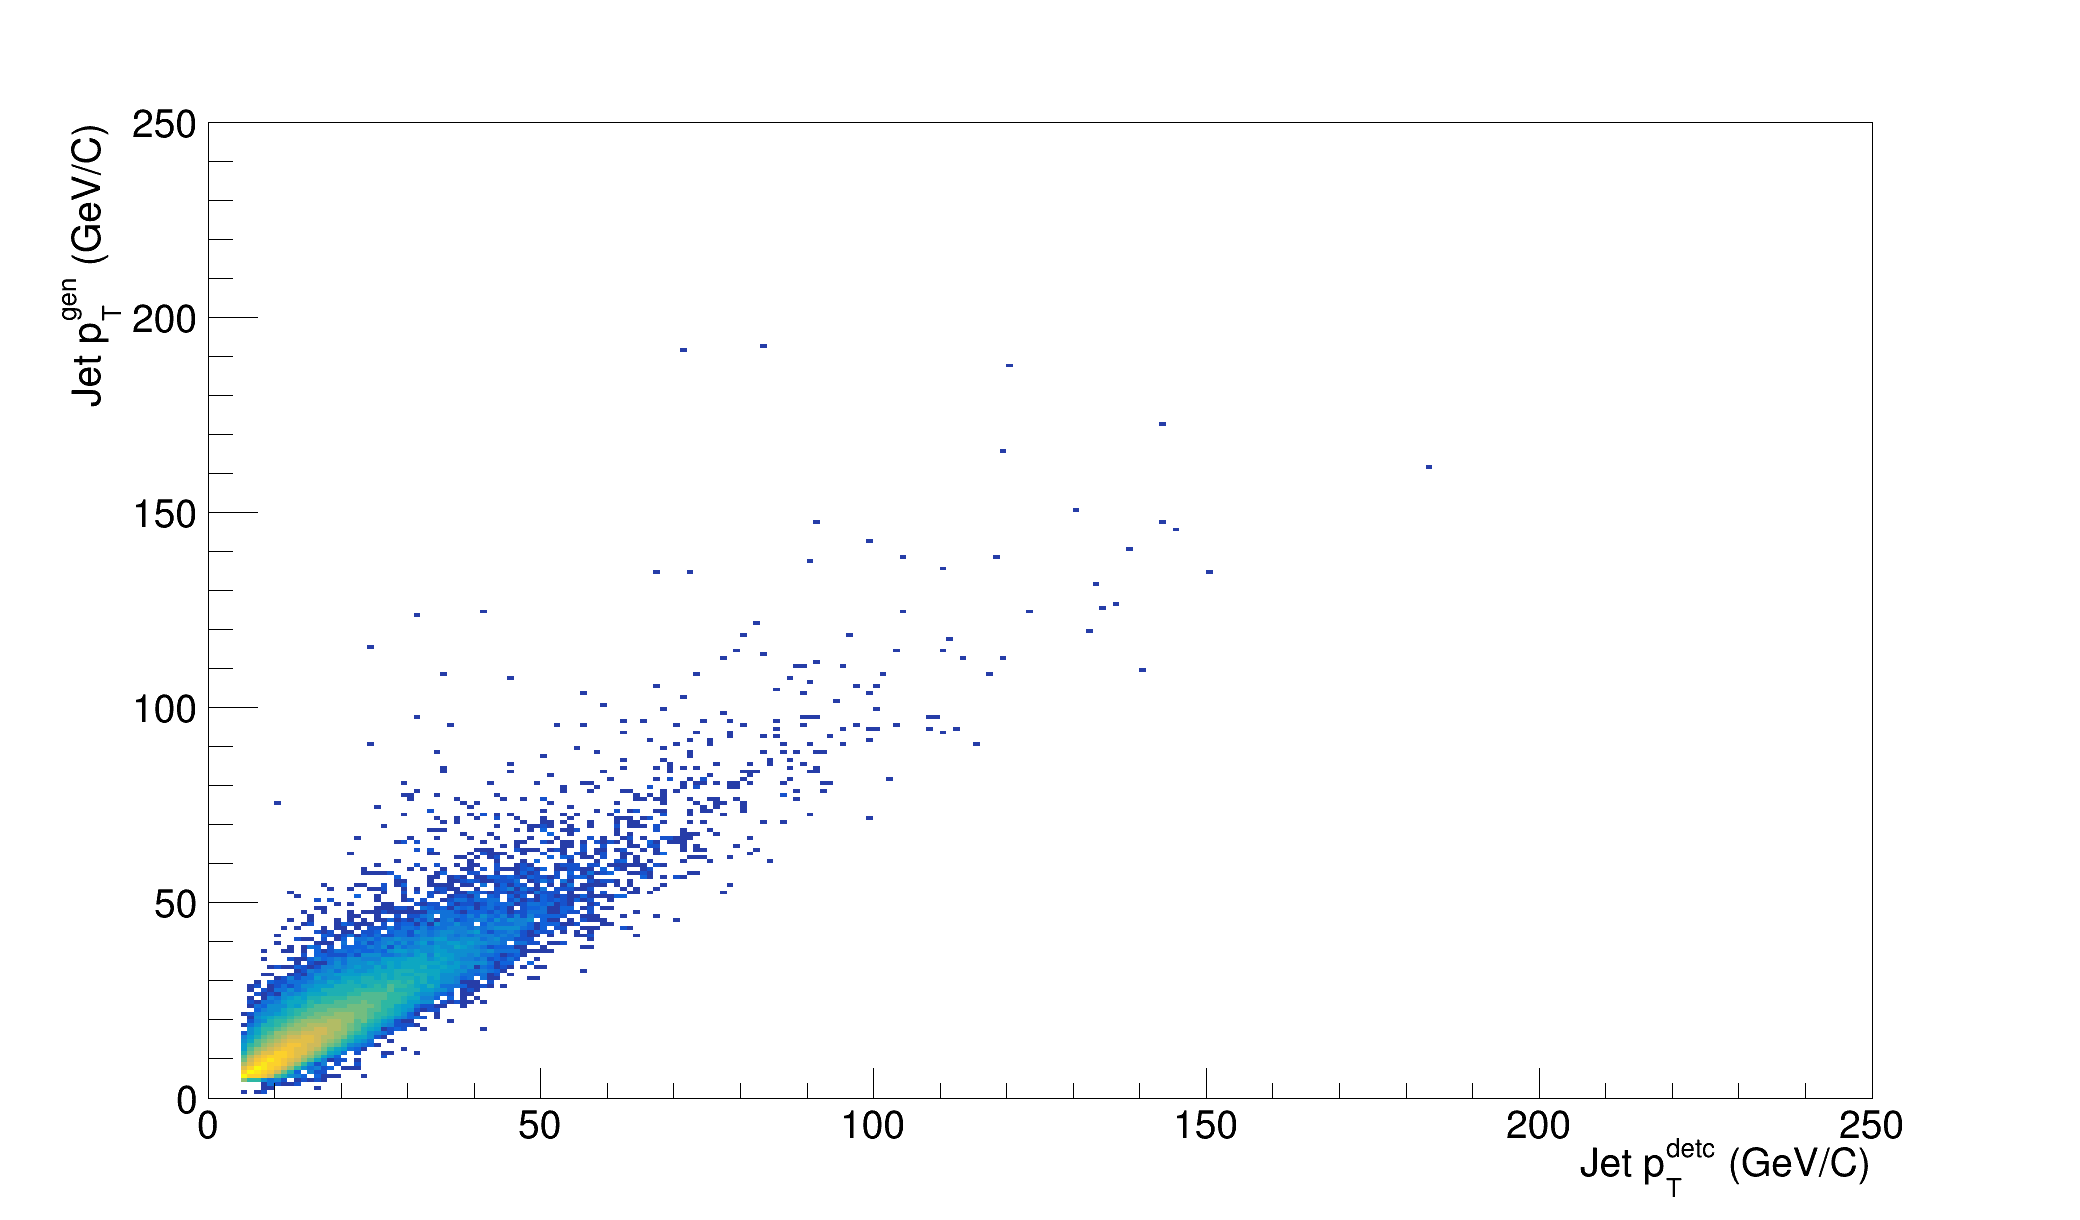
\includegraphics[width=0.5\textwidth]{responseR04}}
\end{array}$
\caption[Response Matrices for R = 0.2, R=0.3, and R = 0.4 jets.]{\label{fig:response}Response Matrices for R = 0.2, R=0.3, and R = 0.4 jets.}
\end{figure*}

Figure \ref{fig:response} shows the response matrices for the R = 0.2, R = 0.3, and R = 0.4 jets generated with the prescribed manner.  The response matrices display a linear relationship below 50 GeV on both axis and show that above $\sim$100 GeV the matrices are statistically starved.  This is primarily because the Monte Carlo Pythia and PHOJet data sets generated for the 8 TeV pp run did not model the high-$p_{T}$ triggers associated with the EMCal.  The particle jet finders configured for the response matrices allowed for jet finding down to a 100 MeV jet candidate at the particle level with no constraints on the minimum particle momentum or energy for a constituent.  The detector level jet finders were configured in the same manner as they were for the raw jet spectra measurement.  

\subsubsection{Corrections to Particle Level}

Unfolding was performed using the \verb+RooUnfold+\cite{Adye:2011gm} software package.  Corrections were applied using the bin-by-bin\cite{Cowan:2002in} algorithm. 

\begin{equation}
C_{MC} \big( p_{T}^{low} : p_{T}^{high} \big) =  \frac{  \int^{p_{T}^{high}}_{p_{T}^{low}} dp_{T} \; \frac{dF^{uncorr}_{meas}}{dp_{T}} \times \frac{d^{2}N^{particle}_{MC}/d\eta \, dp_{T}}{d^{2}N^{detector}_{MC}/d\eta \, dp_{T}}  } { \int^{p_{T}^{high}}_{p_{T}^{low}} dp_{T} \; \frac{dF^{uncorr}_{meas}}{dp_{T}} }
\label{eq:binbybin}
\end{equation}

\noindent
where $d^{2}N^{particle}_{MC}/dp_{T} \, d\eta$ is the Pythia particle level inclusive jet spectra, $d^{2}N^{detector}_{MC}/dp_{T} \, d\eta$ is the GEANT detector level inclusive jet spectra, $dF^{uncorr}_{meas} / dp_{T}$ is a weight function which minimizes the dependence on the two simulation spectra shapes, and finally $p_{T}^{low}$ and $p_{T}^{high}$ are the lower and upper bin limits.  Due to the limited statistics derived from the Monte Carlos available, the unfolding procedure was stable only in unfolding the truth level jet spectra for the range: $p_{T,jet} \, \epsilon \;$ [10 GeV, 120 GeV] for both the raw Min Bias and EMCal triggered data sets.  The only way to get around this crutch to the analysis would be to ask the ALICE collaboration to make new official particle + detector level simulations that included the EMCal trigger.  The final truth value for the jet spectra will be reported in this range.



\subsubsection{Unfolded Min Bias Spectra}

\begin{figure}[h]
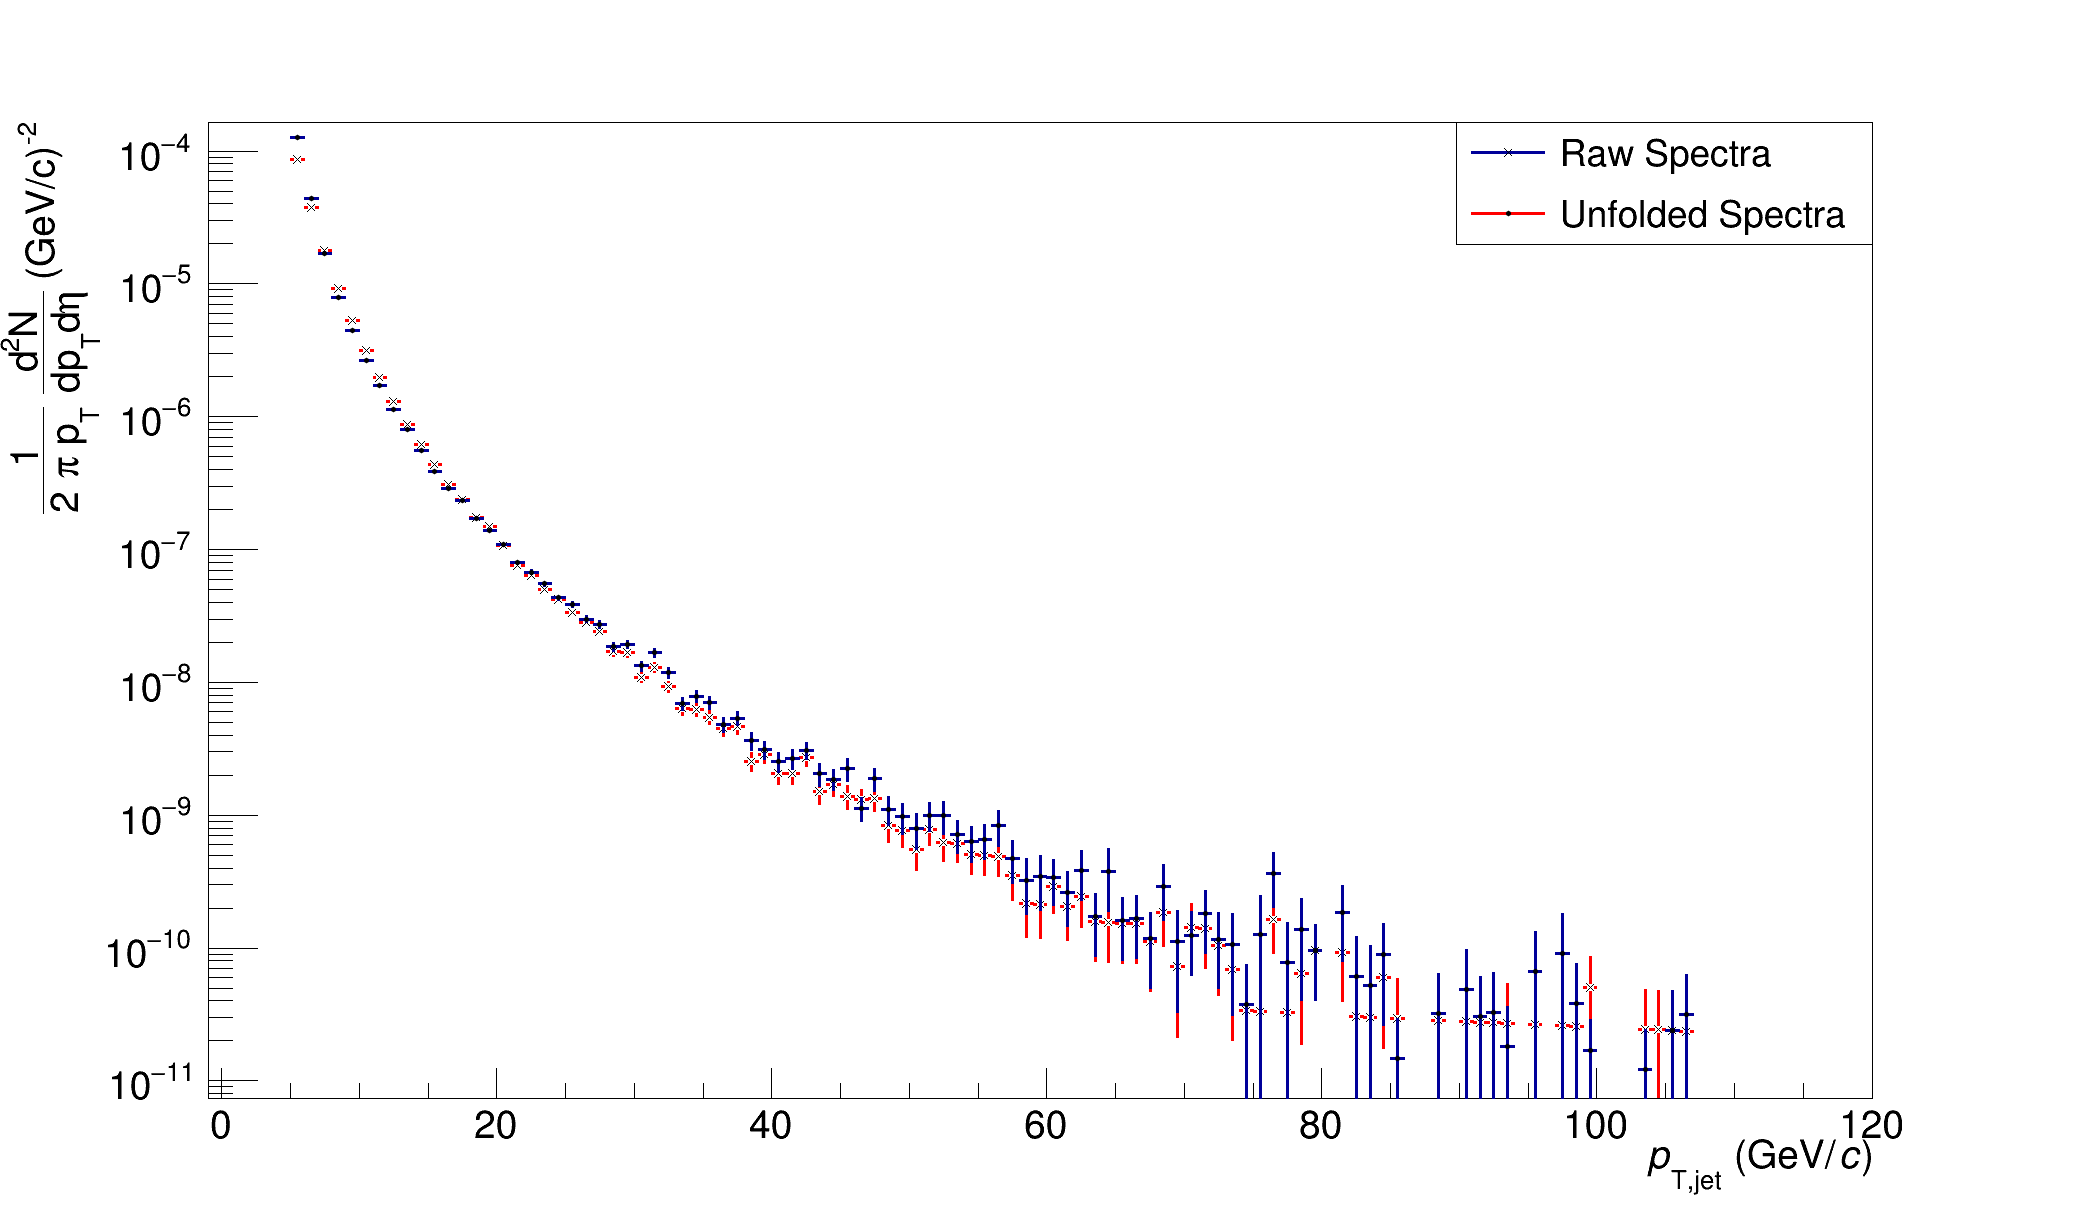
\includegraphics[width=8cm]{RawandUnfoldedSpectraMBR03}
\centering
\caption{Unfolded jet spectra with fine binning for R = 0.3}
\label{fig:Unfoldfine}
\end{figure}

An example of the output from the bin-by-bin unfolding with the fine binning for R = 0.3 jet is shown in Figure \ref{fig:Unfoldfine}.  It should be noted that at low-$p_{T}$ it was observed that unfolding increased the yield of the spectra while at high-$p_{T} \geq \,$ 40 GeV the yield was decreased for all jet radii in this analysis.  This is most likely due to the lack of statistics in the response matrix.  Once the bin-by-bin unfolding has been performed for the fine binned spectra the output along with the bin-by-bin correction factors are rebinned using a variable binning between 10 GeV and 120 GeV, these corrected spectra are shown in Figure \ref{fig:unfoldMinbias}.


\begin{figure*}[t!]
$\begin{array}{rl}
    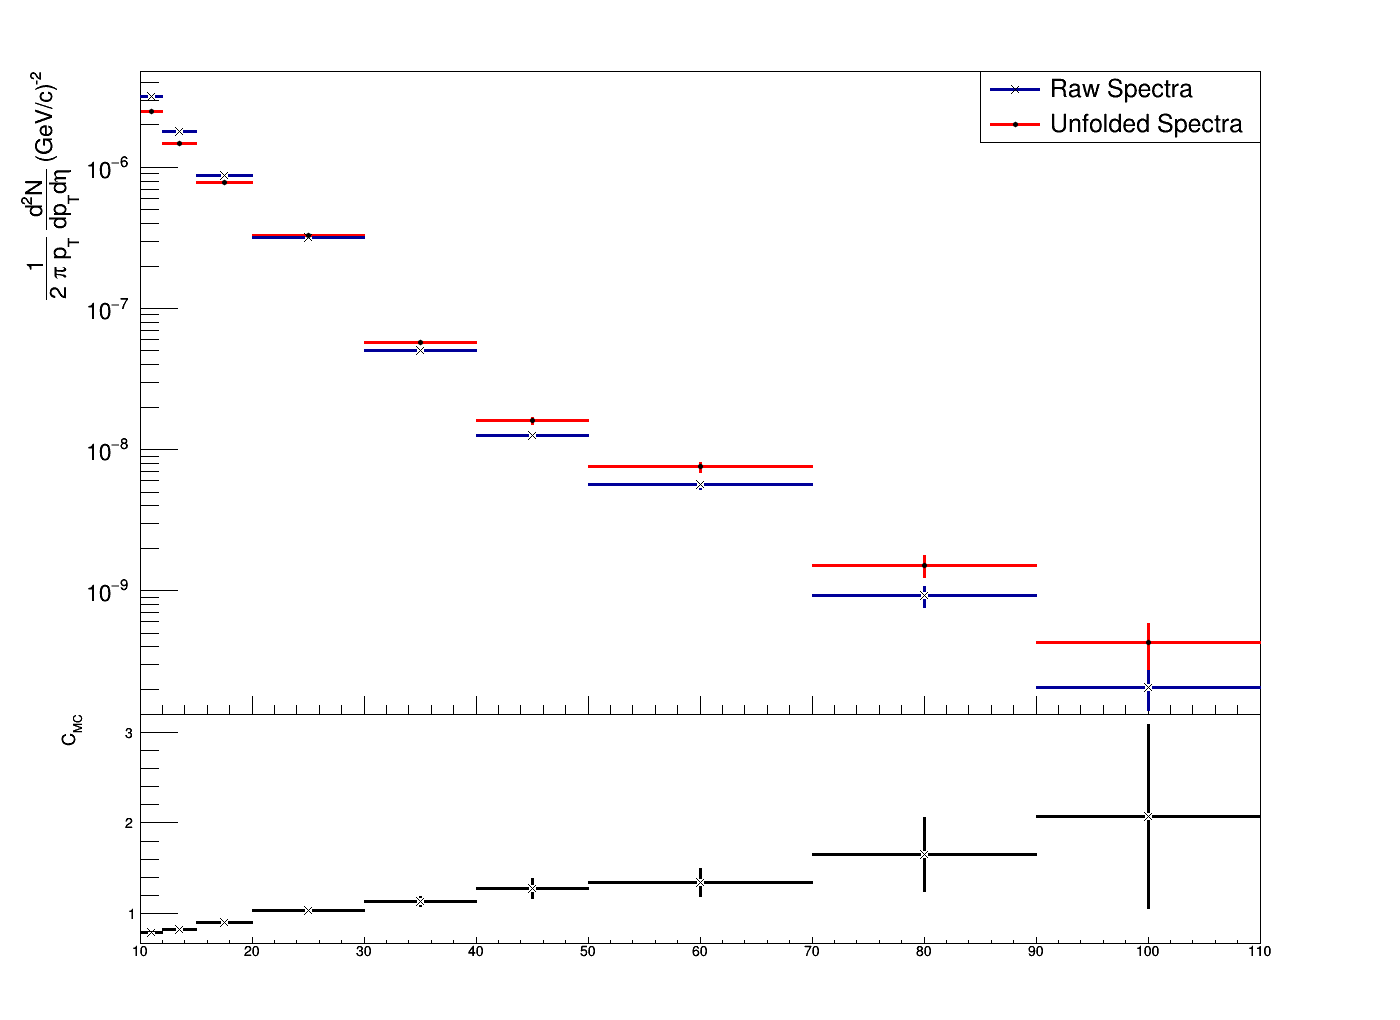
\includegraphics[width=0.5\textwidth]{UnfoldedR02MinBias} &
    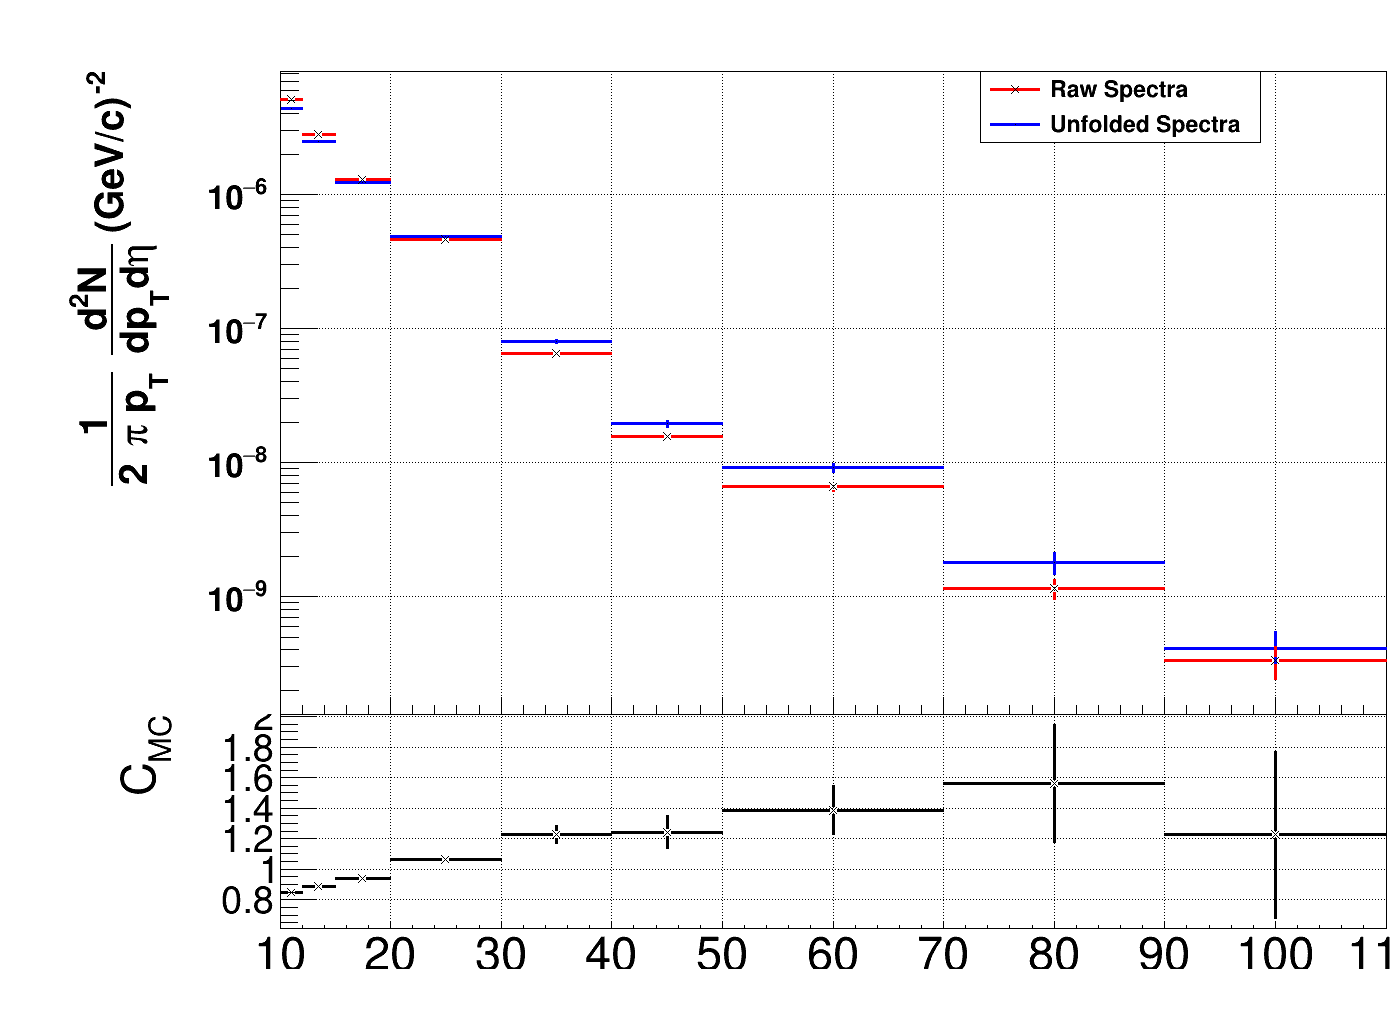
\includegraphics[width=0.5\textwidth]{UnfoldedR03MinBias}\\
    \multicolumn{2}{c}{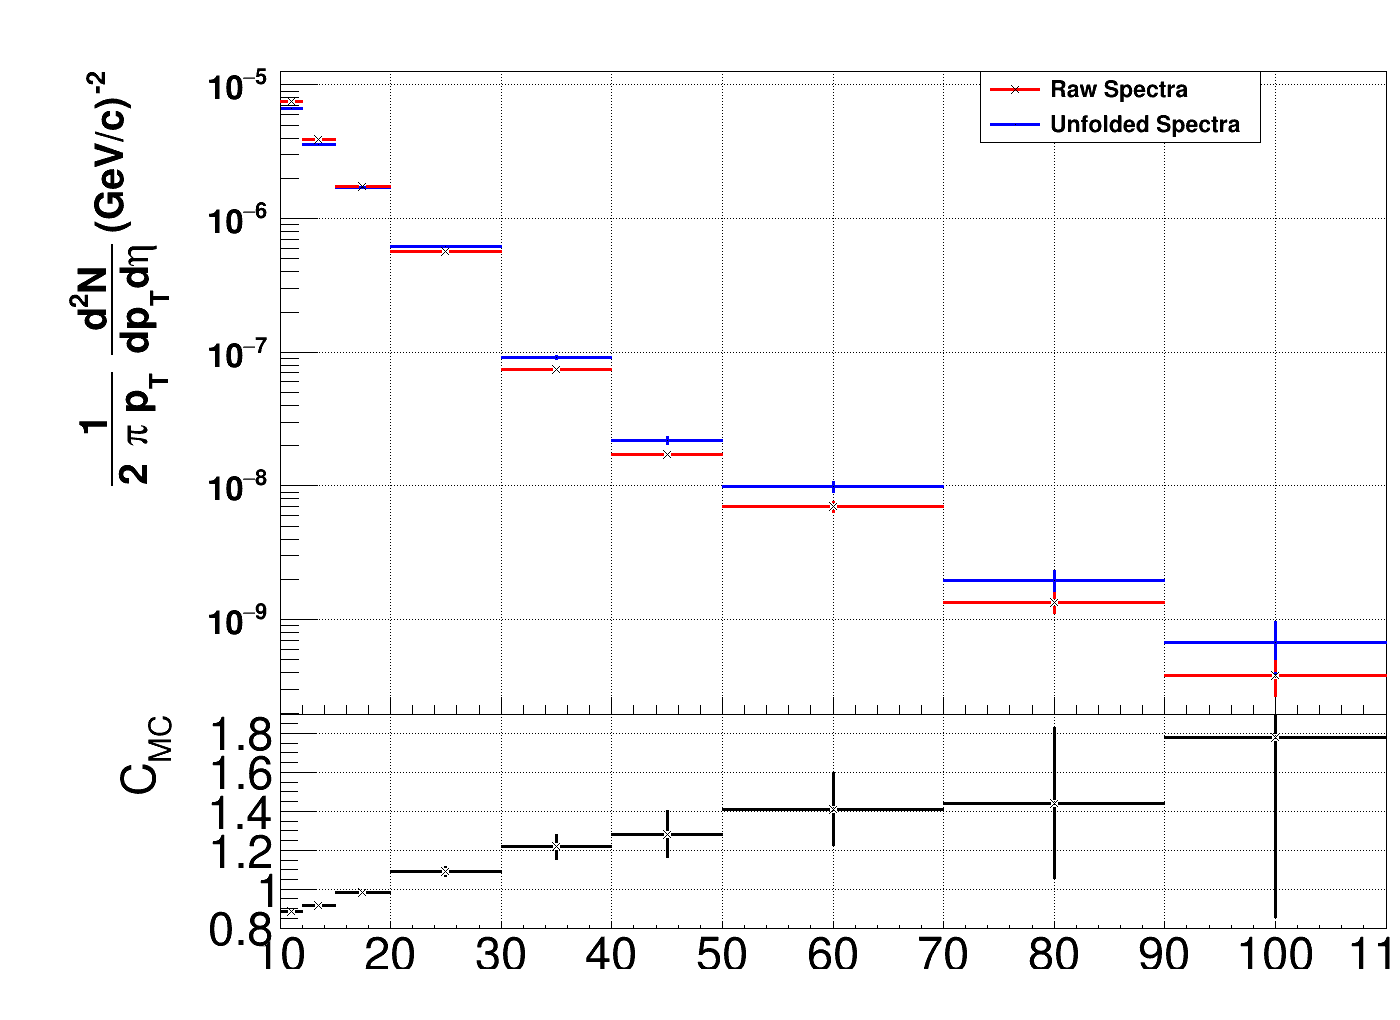
\includegraphics[width=0.5\textwidth]{UnfoldedR04MinBias}}
\end{array}$
\caption[Corrected Jet Spectra to Monte Carlo level for R = 0.2, R=0.3, and R = 0.4 jets.]{\label{fig:unfoldMinbias}Unfolded Min Bias Jet Spectra with correction factors, $C_{MC}$, for R = 0.2, R=0.3, and R = 0.4 jets.}
\end{figure*}

\subsubsection{Unfolded EMCal Triggered Spectra}
The unfolding procedure was repeated again for the EMCal triggered jet spectra.  The response matrix from the Min Bias sample was used for the bin-by-bin unfolding and performed using a fine binning.  The detector level and particle level jets were configured in the same manner as above and the output from the unfolded triggered spectra were reported after rebinning to a variable size over the same kinematic range, as seen in Figure \ref{fig:unfoldEGA}.

\begin{figure*}[t!]
$\begin{array}{rl}
    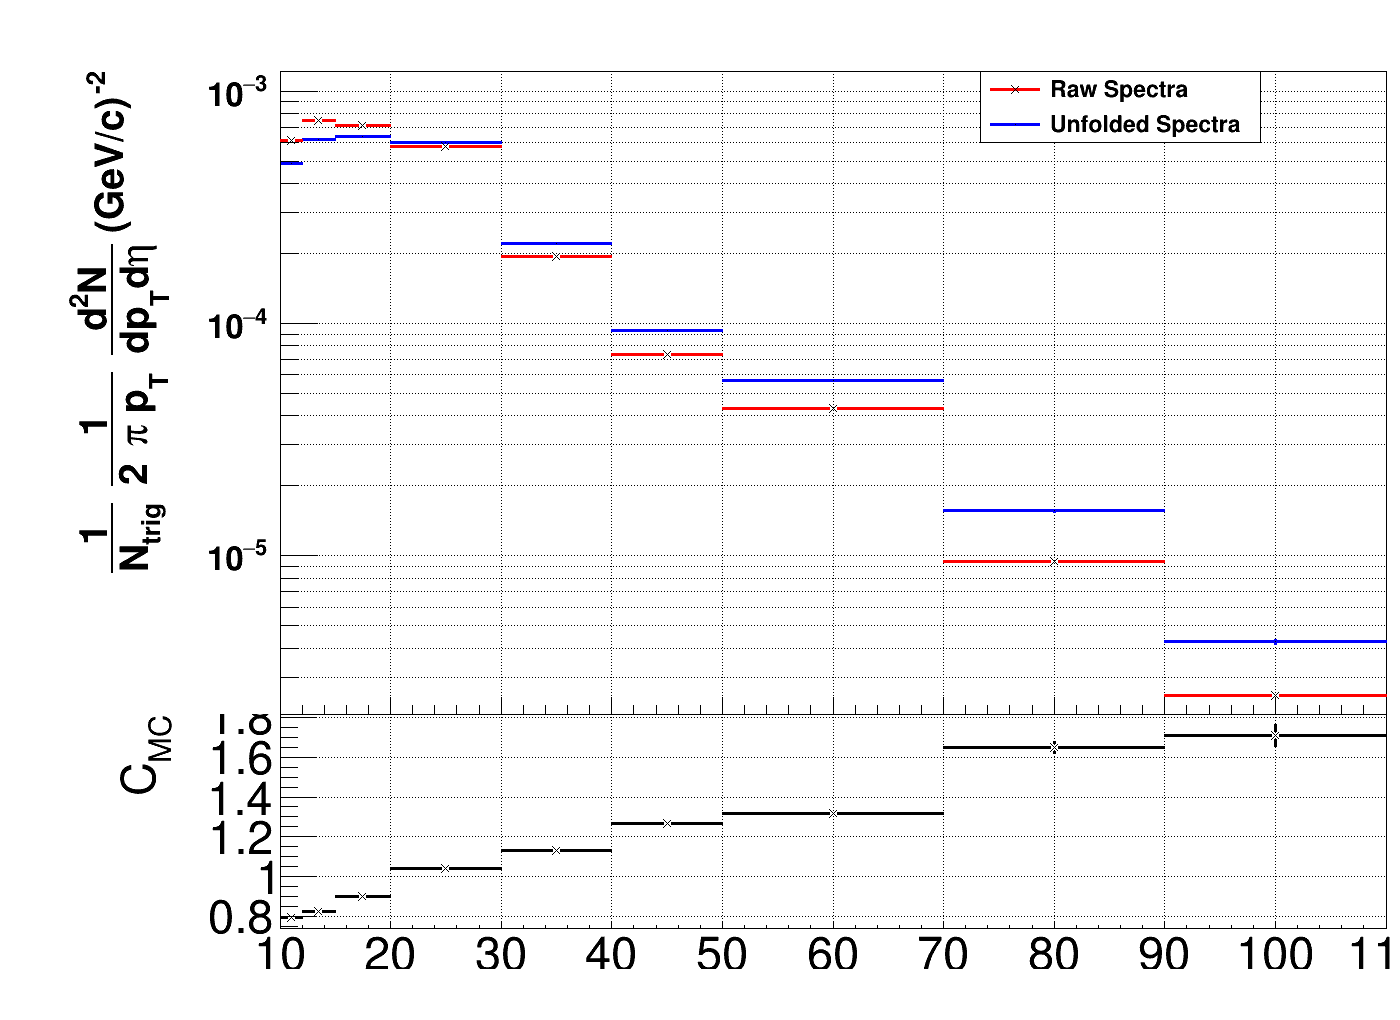
\includegraphics[width=0.5\textwidth]{UnfoldedR02EGAtrigger} &
    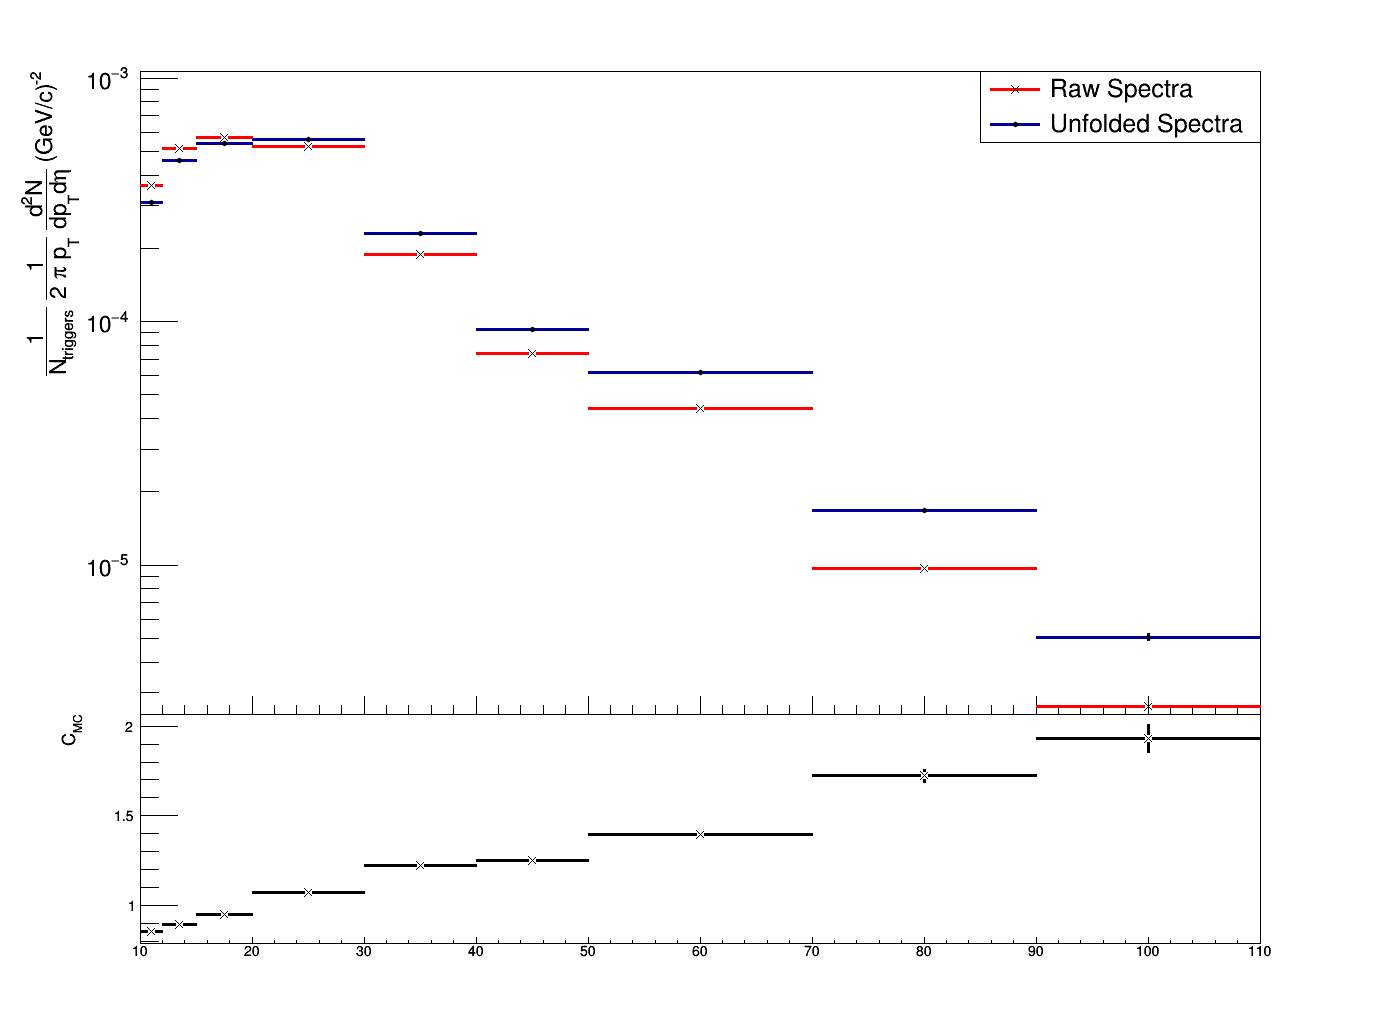
\includegraphics[width=0.5\textwidth]{UnfoldedR03EGAtrigger}\\
    \multicolumn{2}{c}{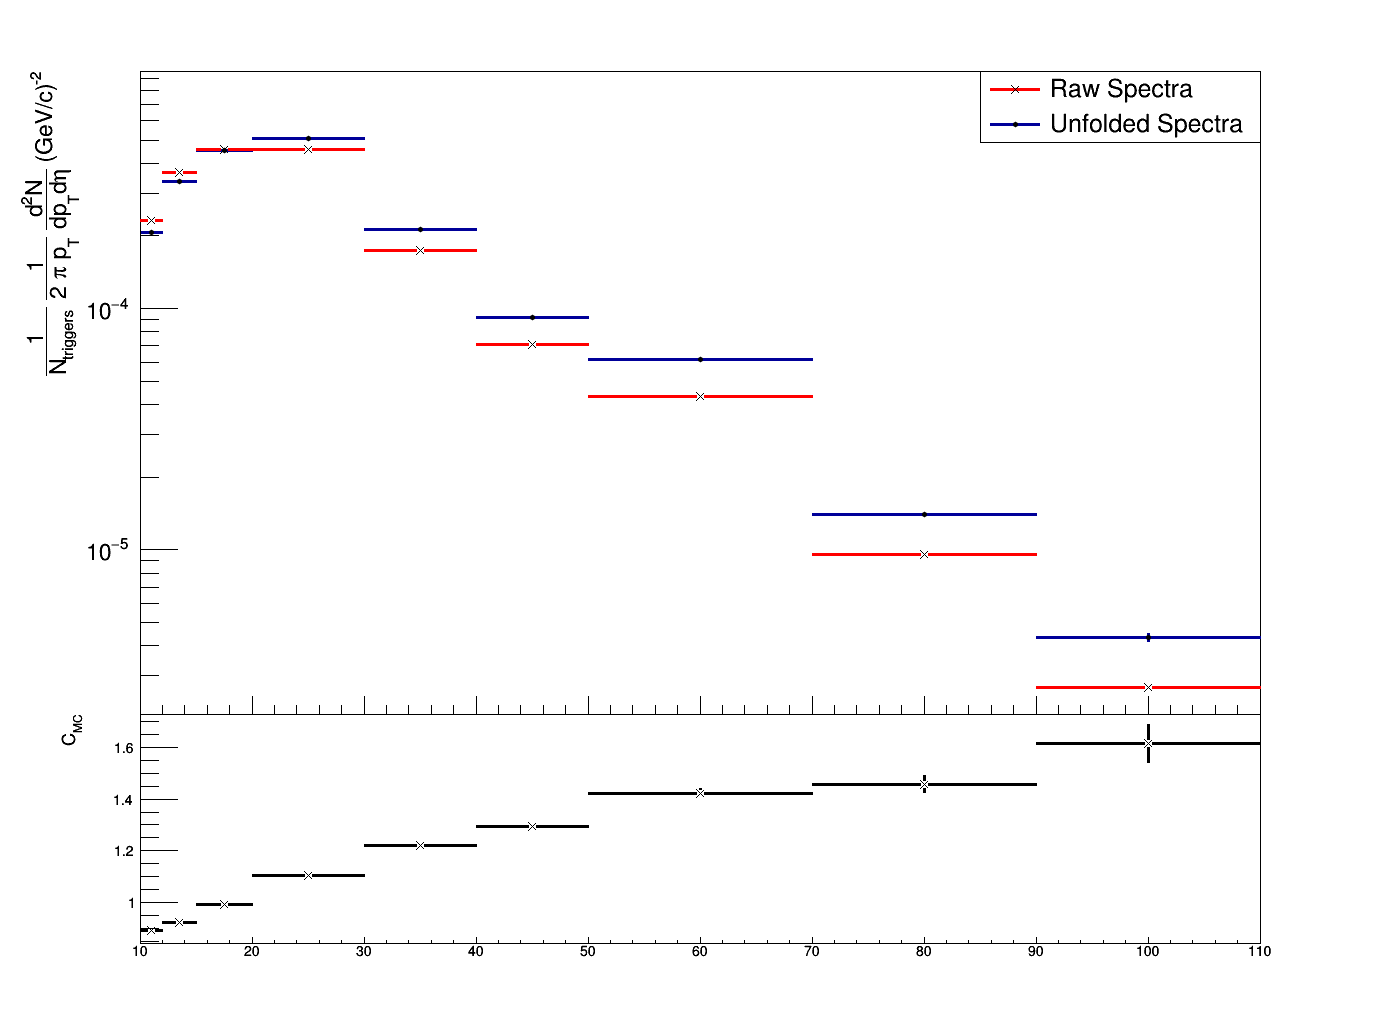
\includegraphics[width=0.5\textwidth]{UnfoldedR04EGAtrigger}}
\end{array}$
\caption[Corrected EMCal Triggered Jet Spectra to Monte Carlo level for R = 0.2, R=0.3, and R = 0.4 jets.]{\label{fig:unfoldEGA}Unfolded EMCal Triggered Jet Spectra with correction factors, $C_{MC}$, for R = 0.2, R=0.3, and R = 0.4 jets.}
\end{figure*}


Due to the limitations of the response matrix, the bin-by-bin unfolding of the EMCal triggered data was only stable up to 120 GeV.  Again, it should be noted that the hump in the EMCal jet spectra is due to the firing threshold of the trigger.  The unfolded EMCal jet spectra was used to estimate the ratio that the jet yields between the Min Bias and triggered data samples, from this point the trigger scaling was calculated.  Due to the lack of a trigger modeled with the 8 TeV Monte Carlo productions, were unable to extend the kinematic range of the jet spectras beyond 120 GeV.  This presents a missed opportunity in terms of the recorded data from the 8 TeV runs.  In order to address this issue a new Monte Carlo production will need to be requested from the ALICE collaboration.

\section{Jet Reconstruction and Matching Efficiency}
In order to quantify the inefficiencies due to unfolding along with the inefficiencies in the ALICE experiment in reconstructing jets, we quantify the jet reconstruction efficiency, $\epsilon_{reco} (p_{T, jet})$, and the jet matching efficiency, $\epsilon_{match} (p_{T, jet})$.

\begin{equation}
 \epsilon_{reco} (p_{T, jet}) = \frac{N_{reco}(p_{T, jet}) }{N_{Truth} (p_{T, jet})}
\label{eq:jetrecoeff}
\end{equation}

\begin{equation}
 \epsilon_{match} (p_{T, jet}) = \frac{N_{match}(p_{T, jet}) }{N_{Truth}(p_{T, jet})}
\label{eq:jetmatchoeff}
\end{equation}

\noindent 
where $N_{reco} (p_{T, jet})$ is the reconstructed jet yield at the detector level per $p_{T}$ bin, $N_{match}(p_{T, jet})$ is the reconstructed jet at the detector level that was matched to a particle level jet per $p_{T}$ bin, and $N_{truth} (p_{T, jet})$ is the truth-level particle jet yield from the Pythia embedded event per $p_{T}$ bin.  

The $N_{truth} (p_{T, jet})$ were obtained by running FastJet on Pythia events with no constituent $p_{T}$ cut, while $N_{match}(p_{T, jet})$ and $N_{reco} (p_{T, jet})$ had the same kinematic cuts as the data driven analysis mentioned earlier in this chapter.  The truth level jets contained no geometric acceptance cut in order to account for jets that may have been reconstructed at the detector level, but had no match to a particle level because part of the particle level jet was outside the EMCal acceptance.  The spectrums were corrected by these efficiencies after the bin-by-bin corrections were performed.  The correction factors are shown in Figures \ref{fig:JetMatcheff} and \ref{fig:JetRecoeff}.

\begin{figure*}[t!]
$\begin{array}{rl}
    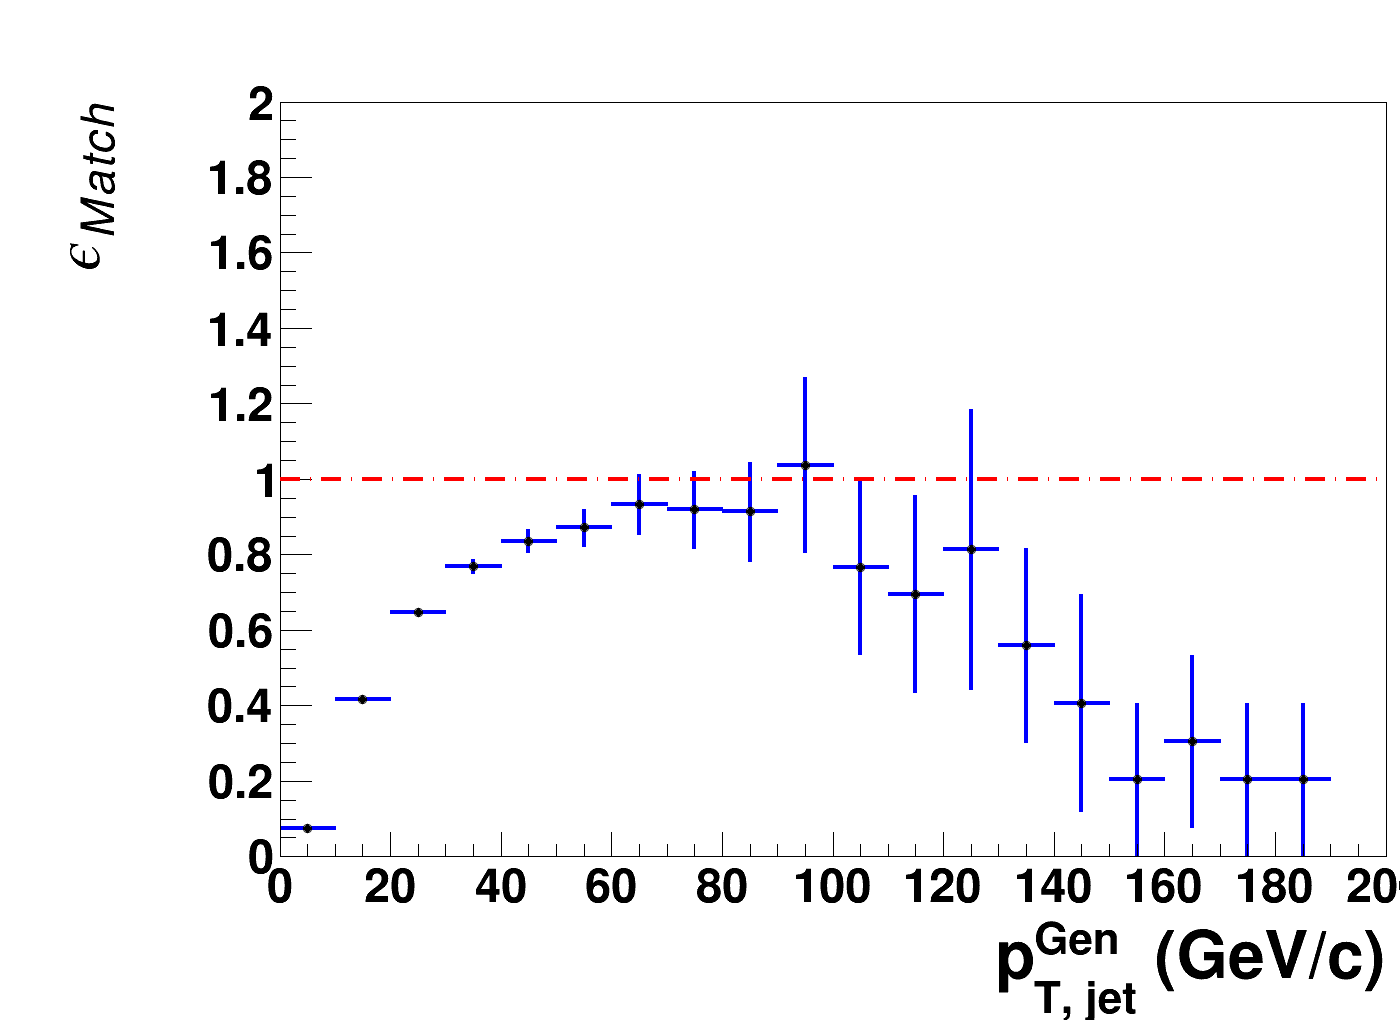
\includegraphics[width=0.5\textwidth]{Ematch_R02} &
    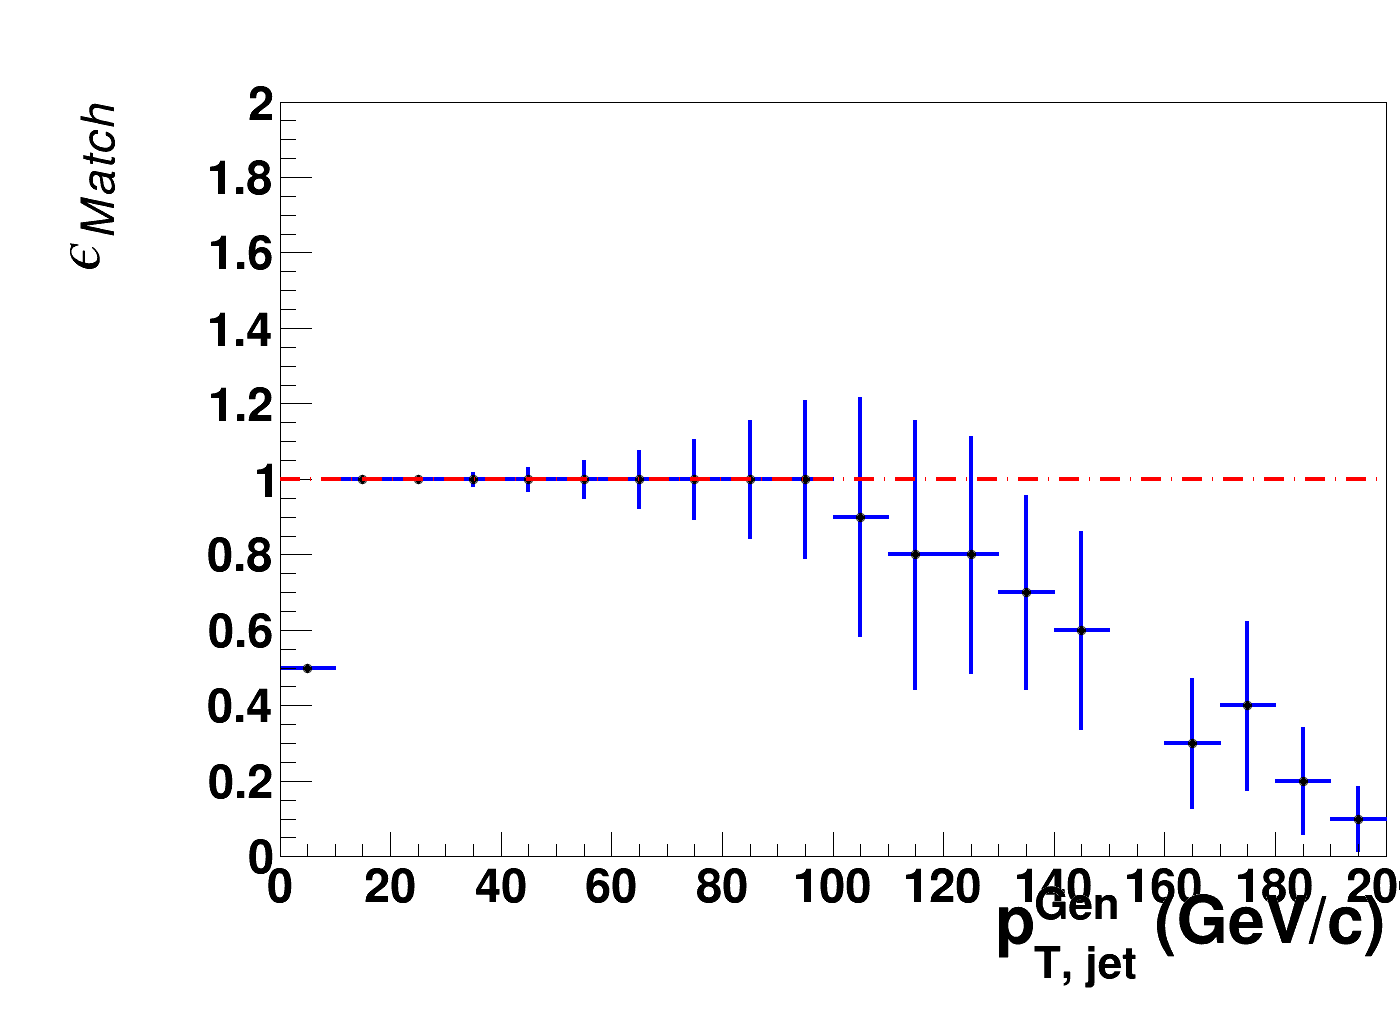
\includegraphics[width=0.5\textwidth]{Ematch_R03}\\
    \multicolumn{2}{c}{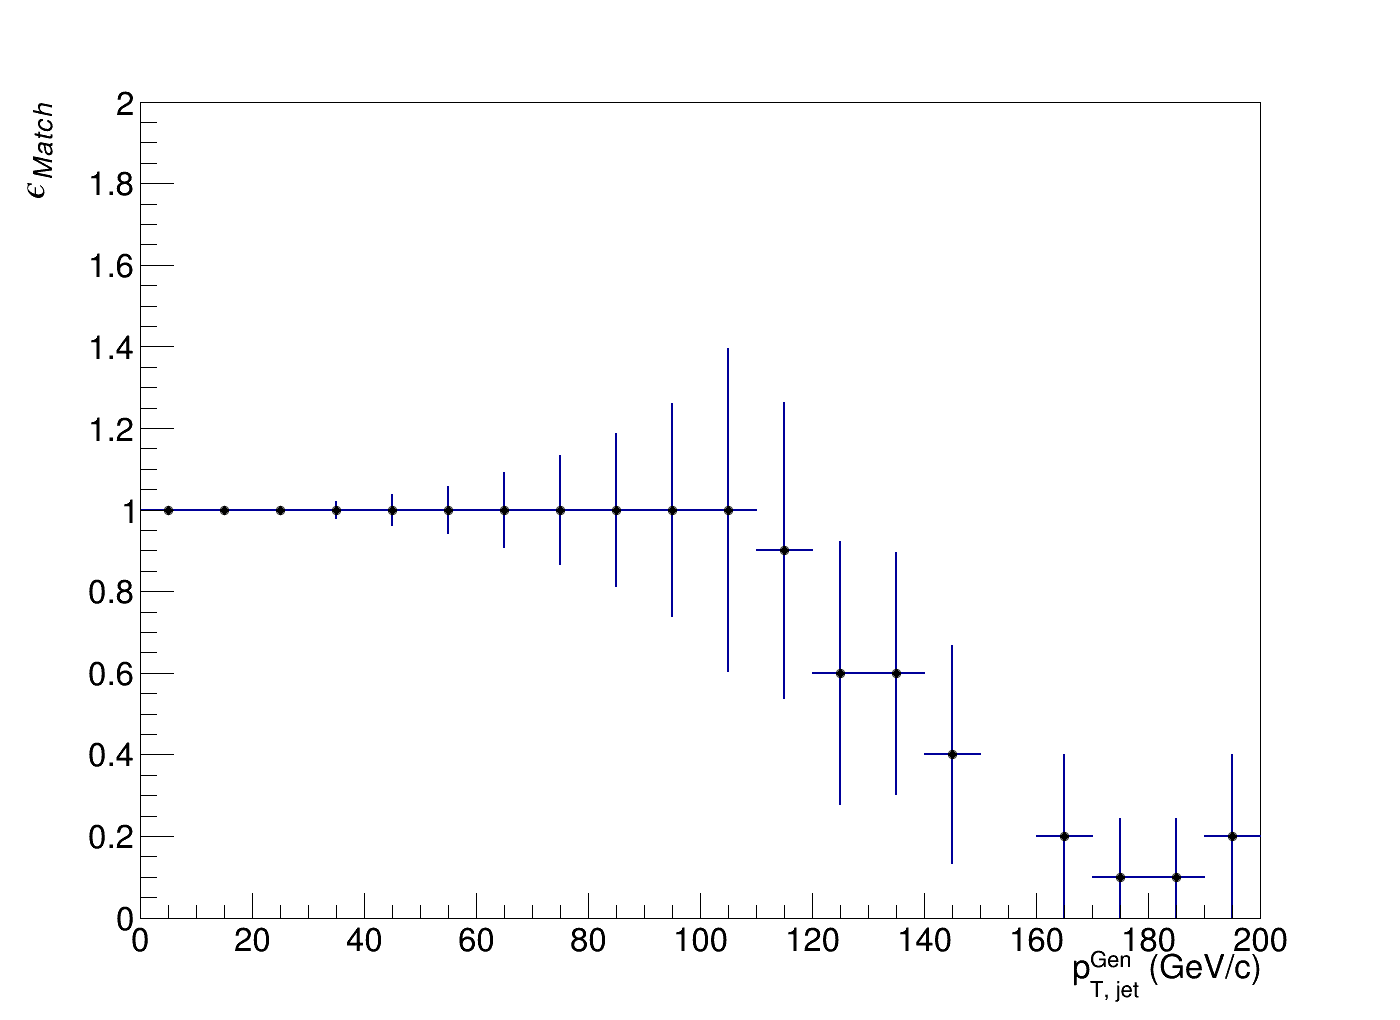
\includegraphics[width=0.5\textwidth]{Ematch_R04}}
\end{array}$
\caption[Jet reconstruction efficiency for jets between R = 0.2 and R = 0.4. ]{\label{fig:JetMatcheff}Jet matching efficiency for jets between R = 0.2 and R = 0.4.}
\end{figure*}

\begin{figure*}[t!]
$\begin{array}{rl}
    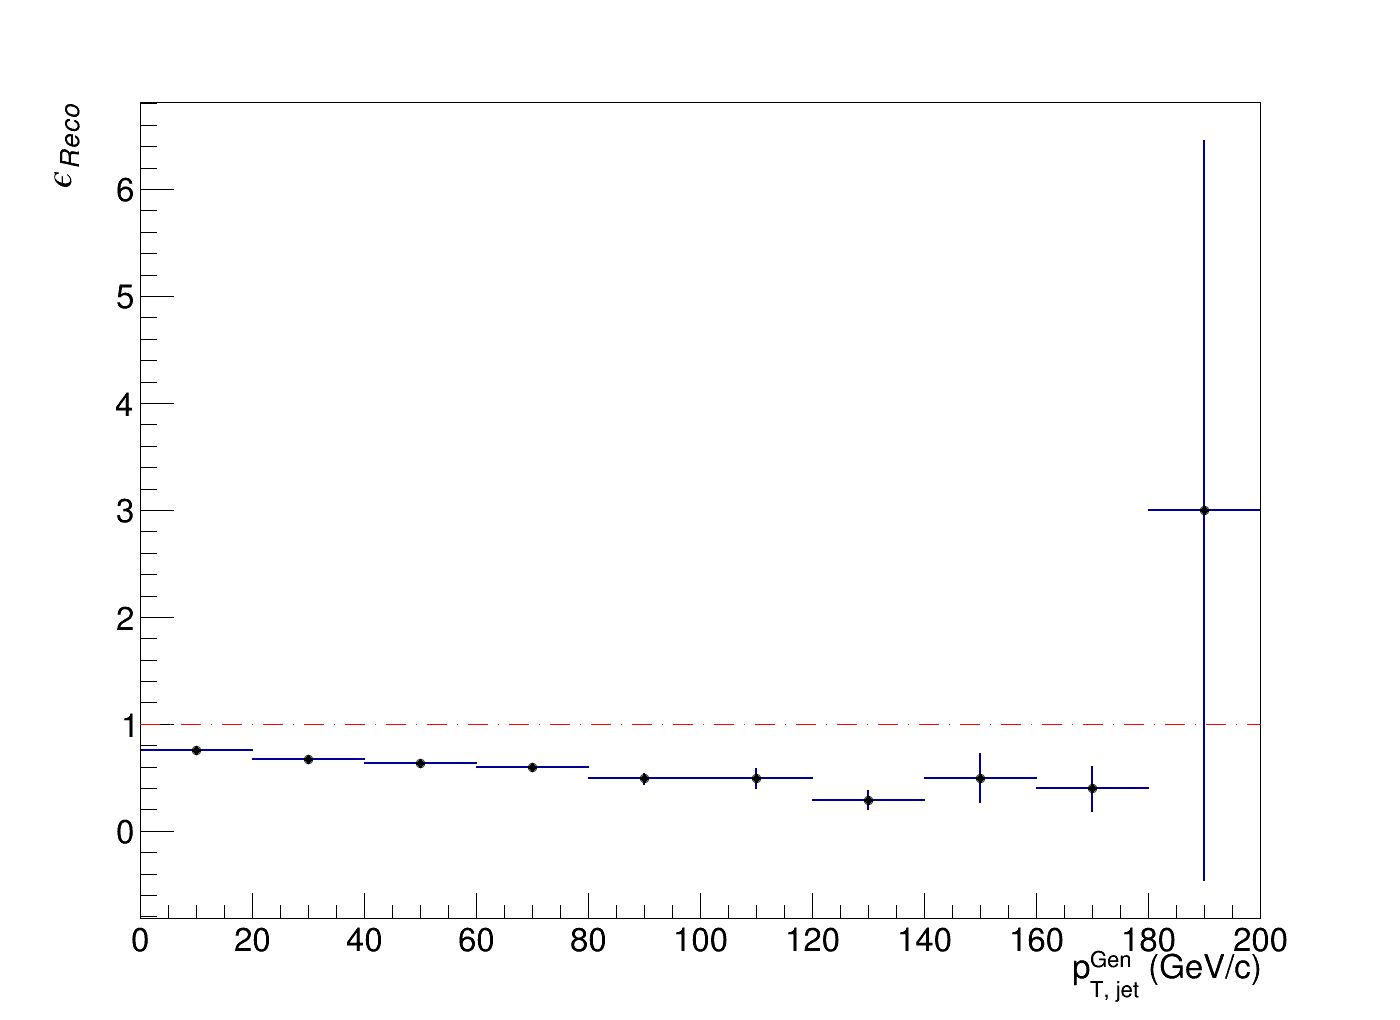
\includegraphics[width=0.5\textwidth]{Ereco_R02} &
    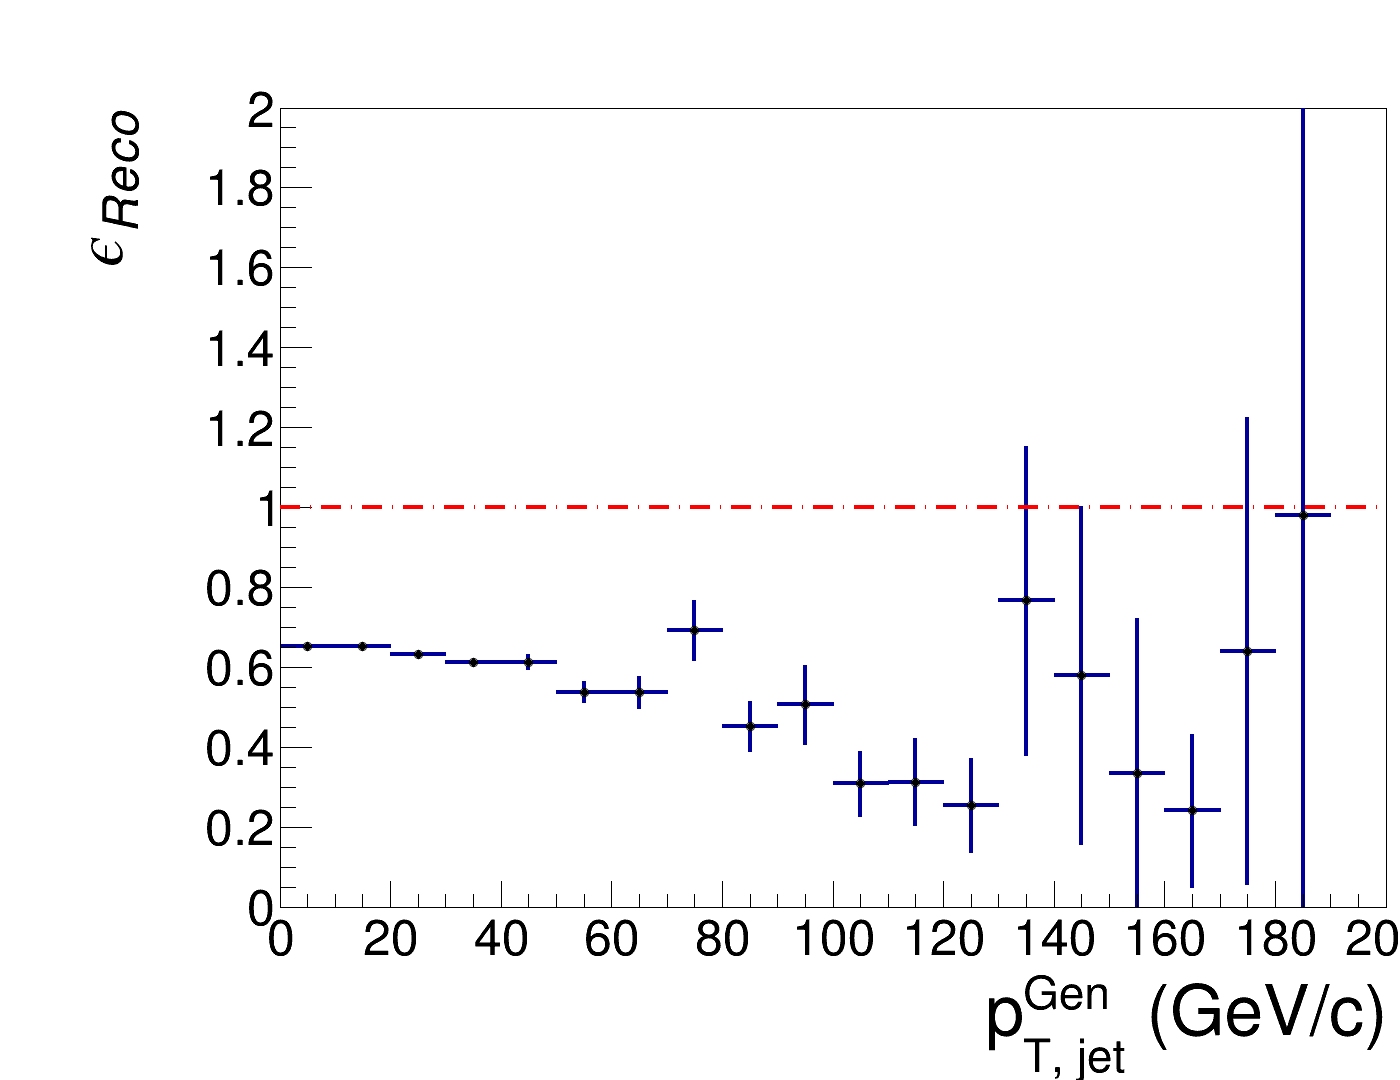
\includegraphics[width=0.5\textwidth]{Ereco_R03}\\
    \multicolumn{2}{c}{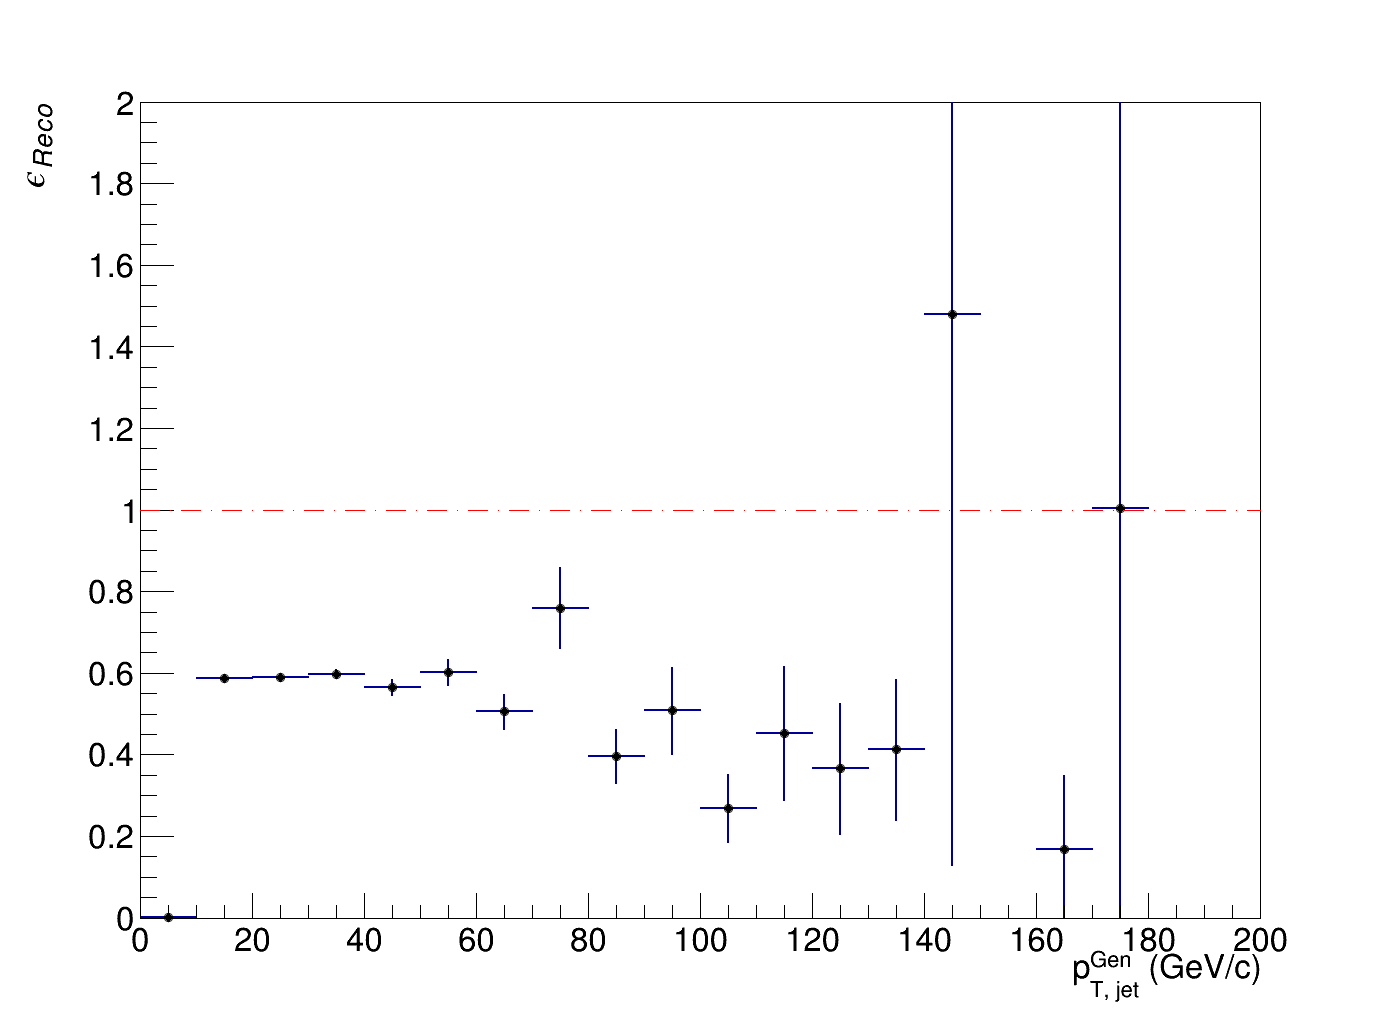
\includegraphics[width=0.5\textwidth]{Ereco_R04}}
\end{array}$
\caption[Jet reconstruction efficiency for jets between R = 0.2 and R = 0.4.]{\label{fig:JetRecoeff}Jet reconstruction efficiency for jets between R = 0.2 and R = 0.4}
\end{figure*}


.

\section{Systematic Uncertainties}

The systematics may be broken into two categories: uncertainties in the jet energy scale (JES) which shifts the momentum spectra along the momentum axis, and uncertainties in the jet yield, which shift the spectra along the spectra/cross-section axis.  The systematical and statistical uncertainties presented in this analysis will be reported as errors to the yield of the spectra. 
 Due to the fact that the $p_{T}$ distribution follows a power law function, $d\sigma/dp_{T} \sim p_{T}^{-5}$ uncertainties to the JES are converted to yield uncertainties by dividing each one by five.
The low statistics at the highest $p_{T}$ bins in this analysis mean that uncertainties in this range may have large statistical fluctuations.  Another way to put this is that small systematic variations for the input of the jet spectra will have a dramatic effect over sparsely filled bins versus bins with a low granularity.  As such it may be necessary to extrapolate the systematic from a low $p_{T}$ bin to those at the highest $p_{T}$ range.  The systematics were performed on both the Min Bias and EMCal triggered data samples but no large variation was observed between the two, thus only the uncertainties from the Min Bias sample are shown and are extrapolated to the triggered data.


\subsubsection{Systematic Uncertainty to Jet Energy Scale}

The following sections present and discuss the uncertainties caused by shifts to the JES. 

\subsubsection{Tracking Efficiency Sensitivity}
Only a fraction of charged tracks generated by the hard scattering of two protons will be detected in the TPC due to its finite track efficiency.  Uncertainties in the efficiency of the TPC were studied and found to account for a 5\% discrepancy\cite{Abelev:2013ala} between the number of tracks in a collision versus the number of measured tracks in proton-proton collisions.  In order to obtain the error associated with this efficiency, this analysis was reperformed maintaining all the cuts and QA discussed in Chapter \ref{ch:analysis}, while throwing out 5\% of the tracks from each event and remeasuring the jet spectra.  Once this new jet spectra was generated, it was corrected using the bin-by-bin corrections and the ratio of this new spectra was taken with the original spectra to gauge the uncertainty from the tracking efficiency.


\begin{figure*}[t!]
$\begin{array}{rl}
    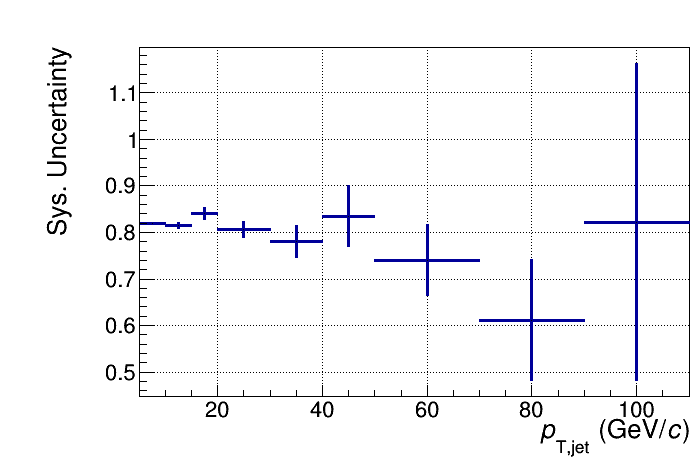
\includegraphics[width=0.40\textwidth]{SysR02_TrkEff} &
    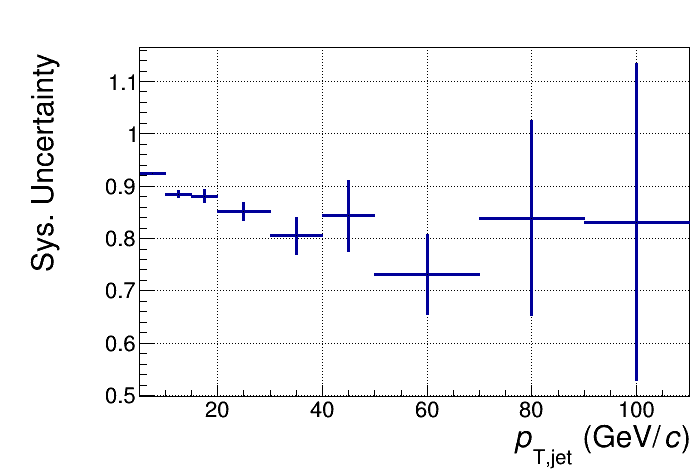
\includegraphics[width=0.40\textwidth]{SysR03_TrkEff}\\
    \multicolumn{2}{c}{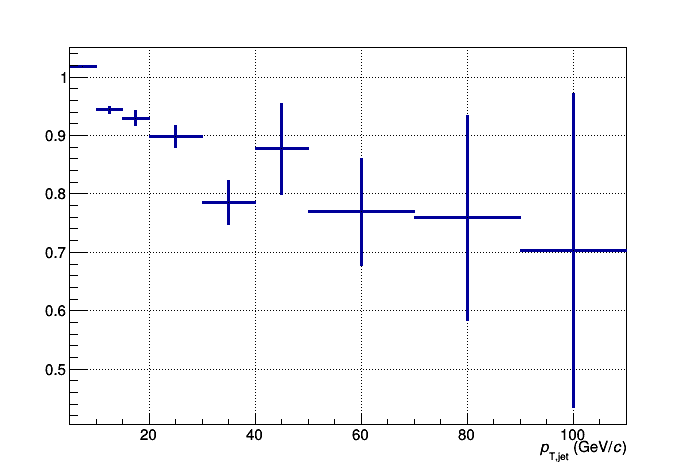
\includegraphics[width=0.40\textwidth]{SysR04_TrkEff}}
\end{array}$
\caption[Systematic due to TPC tracking efficiency.]{\label{fig:trkeff}Systematic due to TPC tracking efficiency; R = 0.2 \textit{(top left)}, R = 0.3 \textit{(top right)}, R = 0.4 \textit{(bottom)}.}
\end{figure*}

\noindent
Figure \ref{fig:trkeff} shows the systematical uncertainties for R = 0.2, R = 0.3, and R = 0.4 jets.  From the figures a 10\% systematic was assigned to R = 0.2 and R = 0.3 jets, while a 15\% systematic uncertainty was given to R = 0.4 jets for this analysis.

\subsubsection{Hadronic Correction}

\begin{figure*}[t!]
$\begin{array}{rl}
    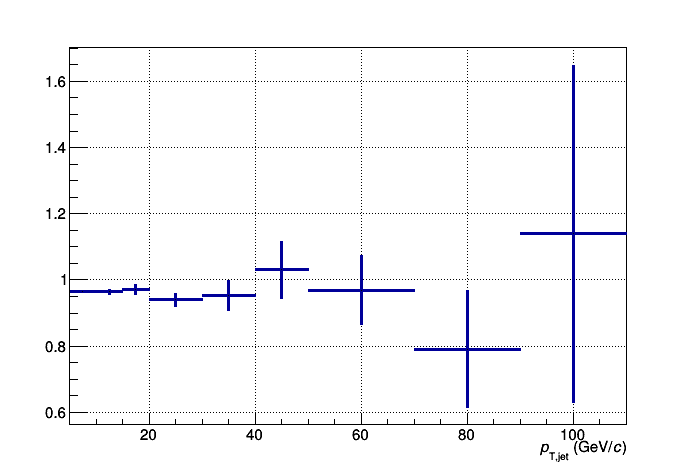
\includegraphics[width=0.40\textwidth]{SysR02_F07} &
    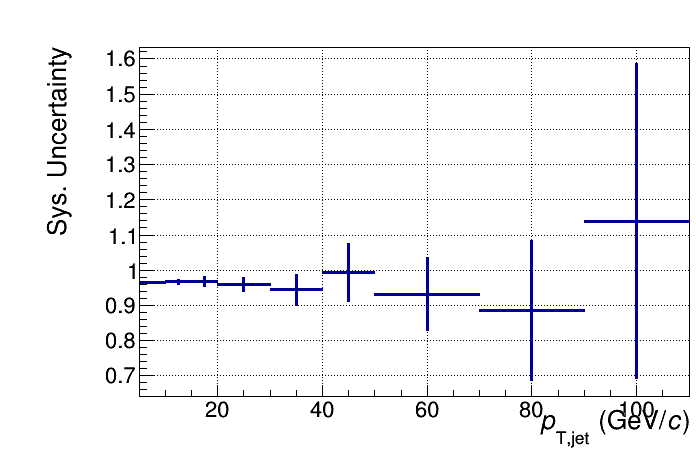
\includegraphics[width=0.40\textwidth]{SysR03_F07}\\
    \multicolumn{2}{c}{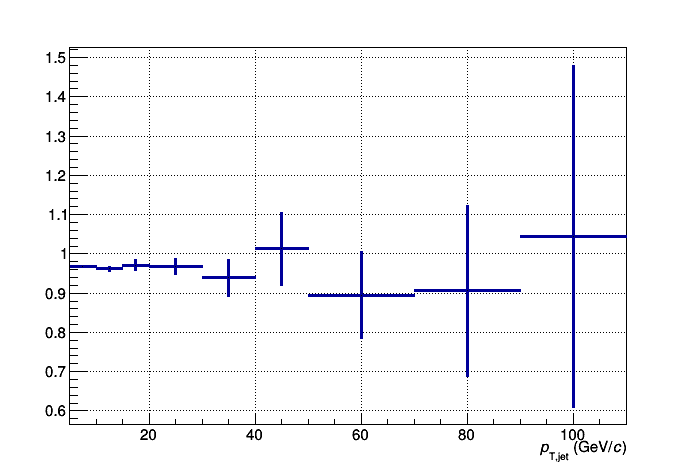
\includegraphics[width=0.40\textwidth]{SysR04_F07}}
\end{array}$
\caption[Systematic due to Hadronic correction.]{\label{fig:hadeff}Systematic due to hadronic correction efficiency; R = 0.2 \textit{(top left)}, R = 0.3 \textit{(top right)}, R = 0.4 \textit{(bottom)}.}
\end{figure*}

In order to assign an uncertainty to the hadronic correction applied to EMCal clusters, the nominal value of $f_{sub} = 1$ in equation \ref{eq:HadCorr} was changed to a value of 0.7 and the analysis chain is repeated.  Figure \ref{fig:hadeff} shows the ratio of the new spectra with the original, and the uncertainty due to the hadronic correction was around 5\% for all jet radii.

\subsubsection{Sensativity to EMCal Clusterization Algorithm}
As previously stated, the clusterizer used in this thesis was the v2 algorithm, which limits the number of EMCal towers in a cluster to a maximum of nine. This algorithm was used in both the detector-level Monte Carlo and data analysis.  In order to test the sensitivity the JES has to the clusterization algorithm, a different algorithm was chosen and a new spectra was generated.  The v1 algorithm was chosen and is similar to the v2 algorithm with the exception that the total size of the cluster is forced to be smaller then nine towers .  Similar to the other systematics presented, we see large anti-correlated variations at high-$p_{T}$ due to sparsely field binning.  

\begin{figure*}[t!]
$\begin{array}{rl}
    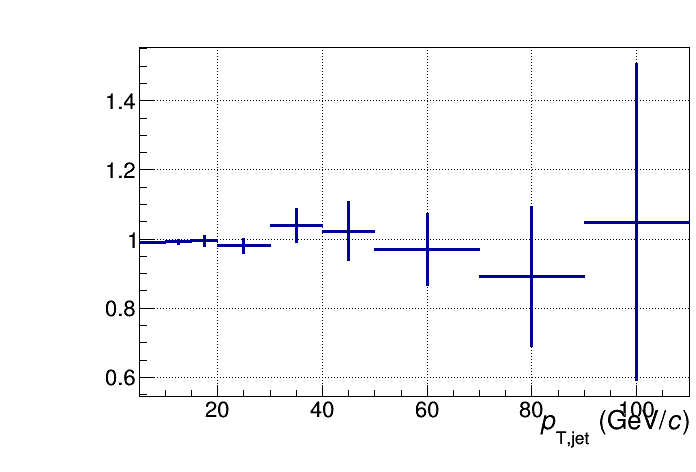
\includegraphics[width=0.40\textwidth]{SysR02_v1Clusterization} &
    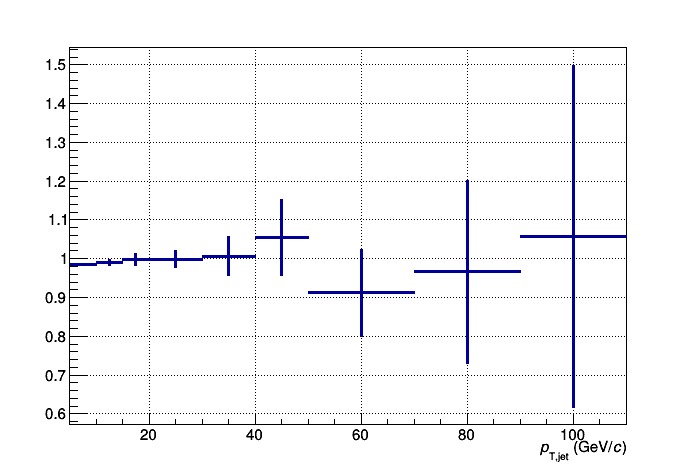
\includegraphics[width=0.40\textwidth]{SysR03_v1Clusterization}\\
    \multicolumn{2}{c}{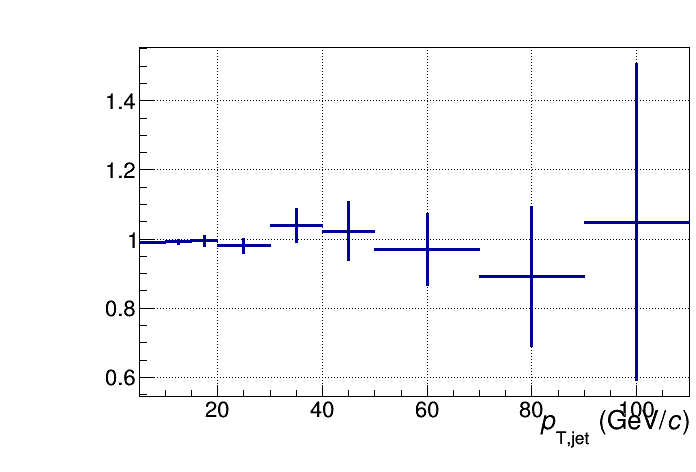
\includegraphics[width=0.40\textwidth]{SysR02_v1Clusterization}}
\end{array}$
\caption[Systematic due to clusterization algorithm.]{\label{fig:cluseff}Systematic due to EMCal clusterization algorithm; R = 0.2 \textit{(top left)}, R = 0.3 \textit{(top right)}, R = 0.4 \textit{(bottom)}.}
\end{figure*}

Figure \ref{fig:cluseff} shows the systematic uncertainty to the clusterization for each of the jet radii.  At low-$p_{T}$ I assigned an uncertainty of between 1\% and 3\% for a given jet radii.  At high-$p_{T}$ I assigned a 5\% for R = 0.2 and 10\% uncertainty for R = 0.3 and R=0.4 jets to help account for the statistical fluctuations.

\subsubsection{Systematic Uncertainty to Jet Yield}

The following sections discuss the systematic uncertainties affecting the jet yield.

\subsubsection{Track $p_{T}$ Resolution}

\begin{figure}[h]
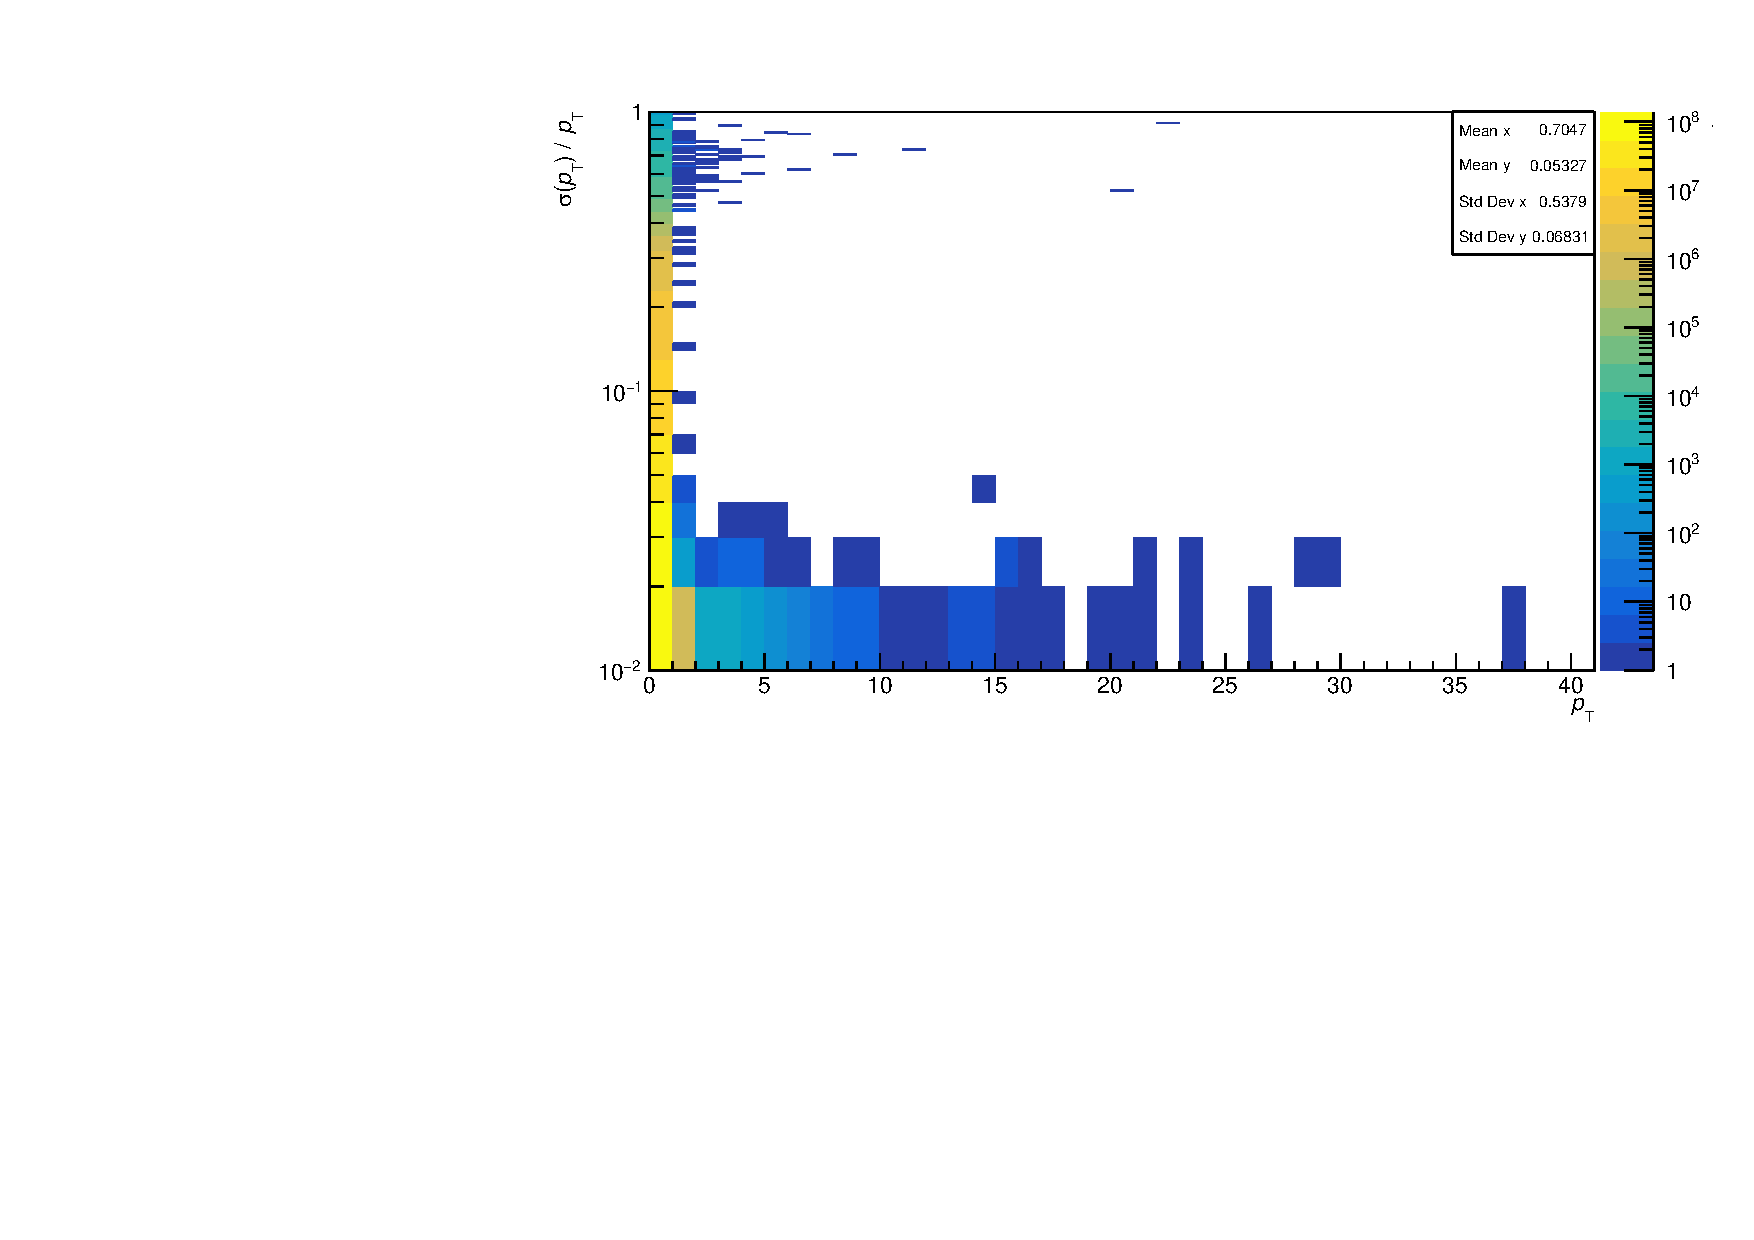
\includegraphics[width=8cm]{trackcovmatrix}
\centering
\caption{Inclusive track resolution, Min Bias 8 TeV.}
\label{fig:trackpcovmatrix}
\end{figure}

\begin{figure*}[t!]
$\begin{array}{rl}
    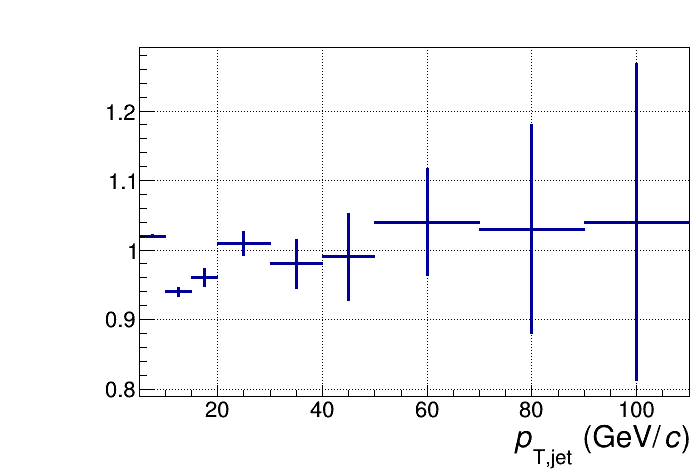
\includegraphics[width=0.40\textwidth]{SysR02_PtReso} &
    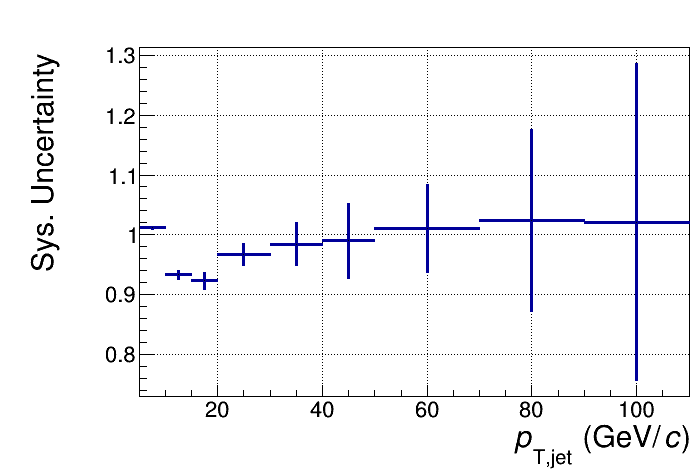
\includegraphics[width=0.40\textwidth]{SysR03_PtReso}\\
    \multicolumn{2}{c}{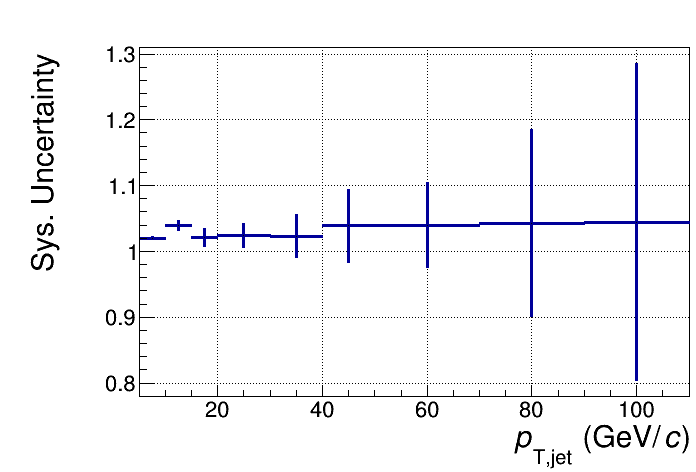
\includegraphics[width=0.40\textwidth]{SysR04_PtReso}}
\end{array}$
\caption[Systematic due to $P_{T}$ resolution.]{\label{fig:pTeff}$P_{T}$ resolution systematic; R = 0.2 \textit{(top left)}, R = 0.3 \textit{(top right)}, R = 0.4 \textit{(bottom)}.}
\end{figure*}

\noindent
The momentum resolution of TPC is estimated using the covariance matrix generated from the Kalman filtering\cite{Fruhwirth:1987fm} pad signal on the TPC read-out region.  Figure \ref{fig:trackpcovmatrix} shows that for the vast majority of the $p_{T}$ range in this analysis the  momentum resolution is below 3\%.  To estimate the systematic due to the $p_{T}$ resolution, tracks are smeared by 3\% in $p_{T}$ and the variation between the new and original spectra are used to estimate the uncertainty.  From the generated plots seen in Figure \ref{fig:pTeff} the uncertainties were below 5\% for all jet radii.

\subsubsection{Cluster Energy Resolution}

\begin{figure*}[t!]
$\begin{array}{rl}
    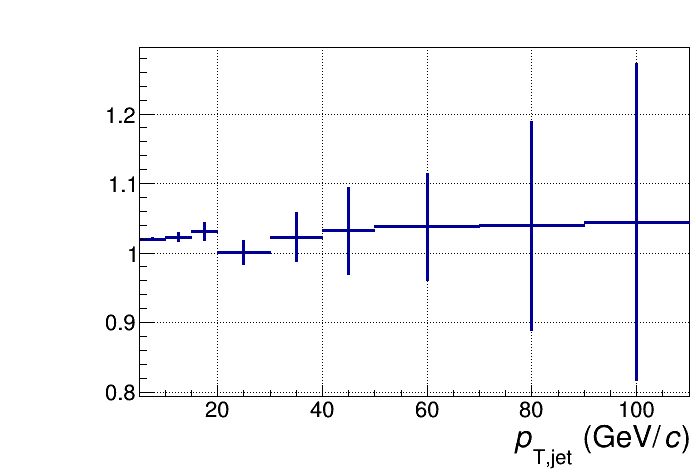
\includegraphics[width=0.40\textwidth]{SysR02_EReso} &
    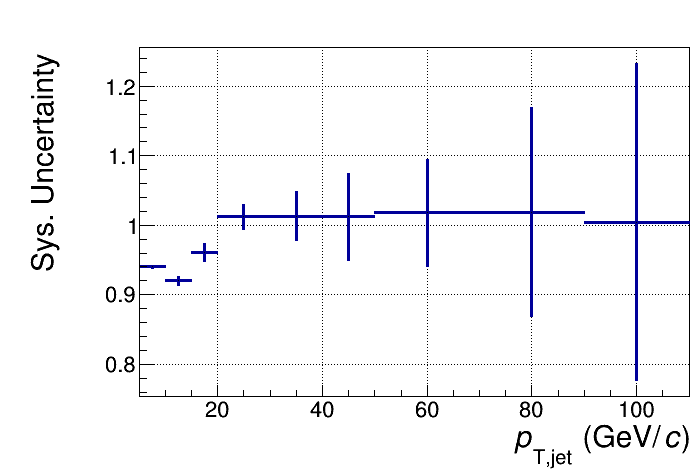
\includegraphics[width=0.40\textwidth]{SysR03_EReso}\\
    \multicolumn{2}{c}{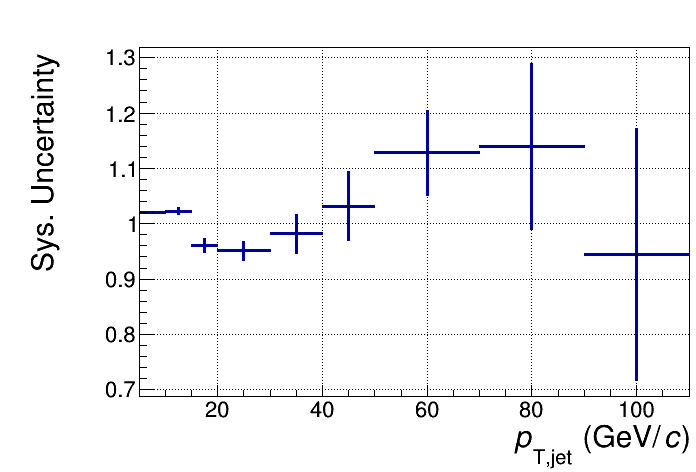
\includegraphics[width=0.40\textwidth]{SysR04_EReso}}
\end{array}$
\caption[Systematic due to energy resolution.]{\label{fig:Eeff}Systematic due to the energy resolution; R = 0.2 \textit{(top left)}, R = 0.3 \textit{(top right)}, R = 0.4 \textit{(bottom)}.}
\end{figure*}

Similar to the $p_{T}$ resolution, the uncertainty due to the EMCal energy resolution is done by smearing the energy of the clusters by the energy resolution function measured from the test beam and seen in Figure \ref{fig:EMCalres}.  The ratio of the spectra with the smear versus the original spectra are show in Figure \ref{fig:Eeff}. The uncertainties for the R = 0.2 and R = 0.3 jets appear well defined and around 1\% - 2\%.  The large variation with R = 0.4 jet energy resolution is due to low statistical fluctuations and a conservative 5\% uncertainty was assigned to this radii.

\subsubsection{Luminosity and Uncertainty}

The luminosity of a hadronic collider, $\mathscr{L}$, is given by the expression



\begin{equation}
\mathscr{L} = \frac{R}{\sigma}
\label{eq:xlumdef}
\end{equation}

\noindent
where R is the interaction rate and $\sigma$ is the visible cross section.  Due to the fact that we only measure events within a 10 cm window within the primary vertex region of ALICE we must scale the total luminosity to that which is delivered within the experiment.  This scale factor is determined by dividing the total number of Min Bias events to those accepted within the 10 cm window.  $N^{tot}_{MB} / N^{10 cm vertex}_{MB}$ = 1.024, which was obtained from the event QA criteria used in this analysis as discussed in Chapter \ref{ch:analysis}.
The total cross-section and luminosity along with there uncertainties were determined during a a special 8 TeV Van der Meer scan run performed in April of 2012\cite{ALICE-PUBLIC-2017-002}.  The total systematic uncertainty for the Min Bias trigger were obtained by measuring the visible cross-section using the T0 and V0 detectors.  The Min Bias trigger was defined as V0AND which required a hit in both the V0A and V0C.  The cross section was reported as being a combined average for Min Bias with the V0AND as, 

\begin{equation}
\sigma_{V0} = (55.8 \pm 1.2) \, mb
\label{eq:xlumdef}
\end{equation}

\noindent
with a combined systematic uncertainty of 2.19\% on the visible cross section and 2.60\% on the luminosity.  Both this cross-section and its uncertainty were scaled by the 1.024 factor to account for the 10 cm vertex region in ALICE before combining with the spectra to obtain the final cross-sections.


\subsubsection{Total Uncertainty}

A summary of the total systematic errors used in the final analysis is given in Table \ref{table:1}.  Some of the uncertainties, for example the $p_{T}$ resolution, used an asymmetric value between the low-$p_{T}$ range, below 40 GeV/\textit{c}, versus high$p_{T}$ range, above 60 GeV/\textit{c}, to account for the statistical fluctuations in the bin filling.  The systematic uncertainties to the yield and JES are added in quadrater together to form the final reported total systematic errors per $p_{T}$ bin.
\newline

\begin{table}[h!]
\centering
\caption{Summary of JES and Yield Uncertainties.}
\begin{tabular}{ |p{5cm}||p{3cm}|p{3cm}|p{3cm}|  }
 \hline
 \multicolumn{4}{|c|}{Systematic Errors} \\
 \hline
 Systematic &R = 0.2 Jets & R = 0.3 Jets& R = 0.4 Jets\\
 \hline
Clusterization (low-$p_{T}$) & 1.0\%    &1.0\%&  3.0\%\\
 (high-$p_{T}$)           &  5.0\%  & 10.0\%   &  10.0\%\\
Hadronic (all bins)&   5.0\% & 4.0\% & 5.0\%\\
Track Eff (low-$p_{T}$)&20.0\% & 15.0\% & 15.0\%\\
 (high-$p_{T}$)            &  25.0\%  & 20.0\%   &  25.0\%\\
Unfolding (all bins)& 6.0\% & 6.0\%&  6.0\%\\
$p_{T}$ Resolution & 2.0\% & 1.0\% & 4.0\%\\
E Resolution& 2.0\%   &1.0\% & 5.0\%\\
Luminosity (all bins) & 2.2\%  & 2.2 \% & 2.2\%\\
 \hline
 \hline
Total Sys (low-$p_{T}$) & 8.9\%  & 6.6\% & 10.9\%\\
(high-$p_{T}$) & 10.3\%  & 9.1 \% & 14.5\%\\
\hline
\end{tabular}

\label{table:1}
\end{table}


